

\chapter{Numerical Methods}\label{Chapter6}
%\blindtext
\minitoc% Creating an actual minitoc

\vspace{5em}


This chapter presents the numerical methods for solving the option pricing problems with transaction costs presented in Section \ref{DPZ_j_sec}.
The optimization problems (\ref{max_probl1}) and (\ref{minimization}) are solved by using the Markov chain approximation method. The same approach has been used 
frequently in the literature in the case of diffusion processes, e.g. \cite{HoNe89}, \cite{DaPaZa93}, \cite{Damgaard}, \cite{Mon04} and \cite{Pal15}. 
We present results for the particular cases of diffusion process, Merton jump-diffusion and Variance Gamma process, although our scheme works for any Lévy process with finite variance. 
We show that our numerical scheme, applied to the problem (\ref{minimization}), is monotone, consistent and stable, and that its solution converges to the viscosity solution of the  
HJB eq. (\ref{HJB2}).
Further analysis, such as numerical convergence rate and time complexity of the algorithm are presented.
In the Section \ref{full_eq_section} are presented numerical results obtained for the general problem (\ref{max_probl1}) where also the default feature is considered.
In the final Section \ref{multinomial_section} we apply the multinomial method introduced in Chapter \ref{Chapter3} to the problem (\ref{minimization}).




\section{Markov chain approximation} \label{MC_section}

In order to solve the problems (\ref{max_probl1}) and (\ref{minimization}) we use the Markov chain approximation method developed by \cite{Kushner}.
The numerical technique for singular controls has been originally developed in the article of \cite{MaKu91}.
The portfolio dynamics (\ref{porfolio_dynamics}) is approximated by a discrete state controlled Markov chain in discrete time. 
The method consists in creating a backward recursive 
dynamic programming algorithm, in order to compute the value function at time $t$, given its value at time $t+\Delta t$.
\cite{Kushner} prove that the value function obtained through the discrete dynamic programming algorithm converges to 
the value function of the original continuous time problem as $\Delta t \to 0$. 
Their proof uses a weak convergence in probability argument.
Another approach to prove convergence has been introduced by \cite{BaSo91}. It consider the convergence of the discrete value function to the viscosity solution of the 
original HJB equation.
In the work of \cite{DaPaZa93} the authors prove existence and uniqueness of the viscosity solution
of the HJB Eq. (\ref{DPZ_HJB}) (diffusion case), and using the method developed by \cite{BaSo91} prove 
that the value function obtained through the Markov chain approximation converges to it.

In this chapter we propose a discretization scheme and prove that it is monotone, consistent, stable, and its solution converges to the continuous viscosity
solution of (\ref{HJB2}).

In this work we model the stock dynamics with a general exponential Lévy process. For practical computations we need to specify
which Lévy process we are using, and this is equivalent to choose a Lévy triplet.
Since every L\'evy process satisfies the Markov property, we are allowed to use the Markov chain approximation approach.  
A possible way to construct the Markov chain is to discretize the infinitesimal generator by using an explicit finite difference method
(see for instance \cite{Kushner} or \cite{FlemingSoner}).
This is straightforward for 
Lévy processes of jump-diffusion type with finite jump activity. 
But for Lévy processes with infinite jump activity, it is not straightforward to obtain the transition probabilities from the discretization of the generator.
A common procedure is to approximate the small jumps with a Brownian motion, as explained in Section \ref{VG_section2}, in order to remove
the singularity of the Lévy measure near the origin. 

\noindent
In the next section we focus our attention on the simplified problem (\ref{minimization}). 


\subsection{The discrete model}\label{discrete_model}

Thanks to the variable reduction introduced in the previous section, the optimization problem (\ref{minimization}) only depends on two state variables. 
The portfolio dynamics (\ref{porfolio_dynamics}) has the simpler form (using $X_t = \log S_t$):
\begin{equation}\label{portfolio_dynamics2}
 \begin{cases}
 dY^{\pi}_t &=  dL_t - dM_t \\
 dX_t &= \biggl( \mu - \frac{1}{2} \sigma^2 - \int_{\R} (e^z-1-z) \nu(dz) \biggr) dt + \sigma dW_t + \int_{\R} z \tilde N (dt,dz).
\end{cases}
\end{equation} 
where the SDE for the log-variable corresponds to (\ref{SDE_log_var}) with $\mu$ defined in (\ref{mu}).
If the process has finite activity $\lambda := \int_{\R} \nu(dz)$, thanks to assumption \textbf{EM} (in Section \ref{AssumptionEM}),
we can define with an abuse of notation\footnote{We have already defined $m$ in (\ref{parameter_m}) and $\alpha$ in (\ref{MertonM}) for the Merton model. 
We extend this notation for any Lévy measure with finite activity.}
$m := \int_{\R} \bigl( e^z -1 \bigr) \nu(dz)$ and $\lambda \alpha := \int_{\R} z \nu(dz)$ such that the SDE of $\{X_t\}_{t \in [t_0,T]}$ can be written as 
\begin{equation}\label{log_sde_fin_act2} 
 dX_t = \biggl( \mu - \frac{1}{2}\sigma^2 -m + \lambda \alpha \biggr) \,dt + \sigma dW_t + \int_{\R} z \tilde N(dt,dz). \\
\end{equation}
If the process has infinite activity $\lambda = \int_{\R} \nu(dz) = \infty$, 
we can approximate the ``small jumps'' martingale component by a Brownian motion, following the arguments in Section \ref{VG_section2}, and get the equation 
\begin{equation}\label{log_sde_inf_act2}
   dX_t = \biggl( \mu - \frac{1}{2} (\sigma^2 + \sigma_{\epsilon}^2) - \omega_{\epsilon} + \lambda_{\epsilon} \theta_{\epsilon}  \biggr) dt + \bigl( \sigma+\sigma_{\epsilon}\bigr) dW_t 
       + \int_{|z|\geq \epsilon} z \tilde N(dt,dz), 
\end{equation}
with parameters defined in (\ref{sig_eps}).

Now we can discretize the time and space to create a Markov chain approximation of the portfolio process (\ref{portfolio_dynamics2}).
For $n = 0,1, ... N \in \N$, we define the discrete time step $ \Delta t := \frac{T - t_0}{N} $ such that
$t_n = t_0 + n \Delta t$.
We assume that the controls $\bigl(L_u,M_u\bigr)$ are constant for $u \in [t_n,t_{n+1})$, and allow for a possible variation at $t_n$ for each $n$.

From now on, we indicate with $X_n$ the value of $X_{t}$ at $t_n$ and with $Y_n$ the value of $Y_{t}$ at the time $t^-_n$ 
immediately before the possible transaction. % we set $t_0 = 0$ and

Let us define the set $\Sigma_x := \{-K_1 h_x , ... , -h_x,0,h_x, ... , +K_2 h_x \}$,  
where $h_x>0$ is the discrete log-return step. The values $K_1,K_2 \in \N$ can be 
different to capture the possible asymmetry in the jump sizes. Its dimension is $\bar L = \#(\Sigma_x) = K_1 + K_2 +1$.
Let us define also the set $\Sigma_y := \{-K_3 h_y , ... , -h_y,0,h_y, ... , + K_4 h_y \} $, 
where $h_y>0$ is the discrete shares step and $K_3,K_4 \in \N$. Its dimension is $\bar M = \#(\Sigma_y) = K_3+K_4+1$.

The discretized version of the SDE (\ref{portfolio_dynamics2}) is: 
\begin{equation}\label{log_sde_discr}
 \begin{cases}
 \Delta Y_n &= \; \Delta L_n - \Delta M_n \\
 \Delta X_n &= \; \hat \mu  \Delta t + \hat \sigma \Delta W_n + \Delta \tilde J_n \; = \; \Delta \Xi_n + \Delta \tilde J_n,
\end{cases}
\end{equation} 
where $\Delta X_n := X_{n+1} - X_{n} \, \in \Sigma_x$, $\hat \mu \in \R$ and $\hat \sigma > 0$. 
The term $\Delta \Xi_n := \hat \mu  \Delta t + \hat \sigma \Delta W_n$ takes values in $\{ -h_x, 0, h_x\}$\footnote{A common alternative is to consider a binomial discretization 
with $\Delta \Xi \in \{-h_x,h_x\}$, as in \cite{DaPaZa93}. }
and satisfies $\E\bigl[\Delta \Xi_n\bigr] = \hat \mu  \Delta t$ and $\E\bigl[(\Delta \Xi_n)^2\bigr] = \hat \sigma \Delta t$, at first order in $\Delta t$.  
%+ \mathcal{O}\bigl(\Delta t^2 \bigr) 
The term $\Delta \tilde J_n$ is the discrete version of the compensated Poisson jump term, and satisfies $\E\bigl[\Delta \tilde J_n\bigr] = 0$ and 
$\E\bigl[(\Delta \tilde J_n)^2\bigr] = \tilde \sigma \Delta t$, at first order in $\Delta t$, with $\tilde \sigma > 0$. 
When the continuous time jump term is $\int_{\R} z \tilde N(dt,dz)$, 
the corresponding discrete version $\Delta \tilde J_n$ can assume all the values in $ \Sigma_x $.
If instead the integral has a truncation term $\epsilon$, i.e. $\int_{|z| \geq \epsilon} z \tilde N(dt,dz)$, we can define the subset 
$ \Sigma^{\epsilon}_x := \Sigma_x \setminus \{ -h_x, 0, h_x\}$, such that $\Delta \tilde J_n \in \Sigma^{\epsilon}_x$.

The Markov chain $\{X_n\}_{n\in \N}$ has the shape of a recombining multinomial tree, where each node has $\bar L$ branches.  
The number of nodes at time $n$ is $n(\bar L-1)+1$.
We derive the transition probabilities by an explicit discretization of the infinitesimal generator (see Section \ref{Markov_Chain2}).
Following \cite{Kushner}, the process $\{X_n\}_{n\in \N}$ has to satisfy the following two conditions in order to be admissible:
\begin{enumerate}
 \item the transition probabilities have the representation:
 \begin{equation}\label{local1}
  p^X \bigl(X_n,X_{n+1}\bigr) = \bigl(1-\lambda \Delta t \bigr) p^{D}\bigl(X_n,X_{n+1}\bigr) + \bigl( \lambda \Delta t \bigr) p^J\bigl(X_n,X_{n+1}\bigr)
 \end{equation}
  where $\lambda > 0$, and $p^{D}$, $p^J$ are respectively the diffusion and jump transition probabilities (see 
  Section \ref{Markov_Chain1}).
 \item (\emph{local consistency}) The moments of the discrete increments match those of the continuous increments, at first order in $\Delta t$: 
\begin{equation}\label{local2}
  \mathbb{E}_n \bigl[ \Delta X_n \bigr] = \mathbb{E}_t \bigl[ \Delta X_t \bigr], \; \quad  %\hat \mu \, \Delta t 
  \mathbb{E}_n \bigl[ ( \Delta X_n )^2 \bigr] = \mathbb{E}_t \bigl[ ( \Delta X_t )^2 \bigr].  % \bigl( \hat \sigma^2 + \tilde \sigma^2\bigr) \, \Delta t
\end{equation}
\end{enumerate}

The process $\{Y_n\}_{n\in \N}$ assumes values in $\Sigma_y$ and $\Delta L_n$, $\Delta M_n$ are non-negative multiples of $h_y$.
The two increments $\Delta L_n := L(t_{n}) - L(t_{n}^-)$ and $\Delta M_n := M(t_{n}) - M(t_{n}^-)$ can occur instantaneously at time $t_n$. 
They cannot assume values different from $0$ at the same time, 
and must satisfy the condition $Y_{n+1} = Y_n + \Delta Y_n \in \Sigma_y$\footnote{The values attainable by $\Delta L_n$ and $\Delta M_n$ 
depend on the current value of $Y_n \in \Sigma_y$. 
For instance, if $Y_n = -K_3 h_y$, then $\Delta L_n \in \{0, h_y, ...,(\bar M-1) h_y \}$ and $\Delta M_n \in \{0\}$.} for all $n$.  




\subsection{Discrete dynamic programming algorithm}\label{algorithm_Sect}
We can formulate a discrete backward algorithm by applying the dynamic programming principle to (\ref{minimization}) 
on the discrete nodes of the chain $\{( Y_n,X_n )\}_n$:
\begin{align}\label{HJB3}
 & Q^{j}(t_n,Y_n,X_n) = \min  
 \; \biggl\{ \E_n \biggl[ Q \bigl( t_{n+1}, Y_n, X_n + \Delta X_n \bigr) \biggr], \\ \nonumber
 & \min_{\Delta L_n} \, \exp \biggl(\frac{\gamma}{\delta(t_n,T)} (1+\theta_b) e^{X_n} \Delta L_n \biggr) 
  \E_n \biggl[ Q^{j} \bigl( t_{n+1}, Y_n+\Delta L_n, X_n + \Delta X_n \bigr) \biggr], \\ \nonumber
 & \min_{\Delta M_n} \, \exp \biggl(\frac{-\gamma}{\delta(t_n,T)} (1-\theta_s) e^{X_n} \Delta M_n \biggr)
  \E_n \biggl[ Q^{j} \bigl( t_{n+1}, Y_n-\Delta M_n, X_n + \Delta X_n \bigr) \biggr]
 \biggr\}.
\end{align}
The variations of $\{Y_t\}_{t \in [t_0,T]}$ are instantaneous at $t_n$ for each $n$, 
while the process $\{X_t\}_{t \in [t_0,T]}$ changes in the interval $[t_n,t_{n+1}]$ according to its Lévy dynamics.
This feature suggests to introduce a numerical scheme based on two steps: an evolution step and a control step.

From now on we drop the superscript $j$ from $Q^j$. We introduce the discretization parameter $\rho = (\Delta t, h_x, h_y)$ and indicate the discretized value function with 
$Q^{\rho}$. For a fixed $\rho$, we adopt the common short notation $Q^n_{j,i} := Q^{\rho}(t_n,y_j,x_i)$. \\
We set the initial value $x_i = X_{n=0}$ for $i=0$. At time $n$, the index $i$ assumes values in 
$\{ -n K_1,-n K_1+1,...,n K_2-1, n K_2 \}$ and $j$ assumes values in $\{ -K_3, -K_3+1,..., K_4-1, K_4 \}$.   

We can define the auxiliary functions: 
\begin{align}\label{FG}
& F(x_i,l,t_n) := e^{\bigl(\frac{\gamma}{\delta(t_n,T)} (1+\theta_b) e^{x_i} lh_y \bigr)}  \\ \nonumber
& G(x_i,m,t_n) := e^{\bigl(- \frac{\gamma}{\delta(t_n,T)} (1-\theta_s) e^{x_i} mh_y \bigr)}, 
\end{align}
such that $l\in \{0,...,K_4-j\}$ and $m\in \{0,...,K_3+j\}$ for each fixed $j$. 
\begin{algorithm}[H] 
\caption{Backward algorithm}
\label{algo}
 \algsetup{indent=1.5em}
 \begin{algorithmic}[1]
    \REQUIRE $r, (b,\sigma,\nu), X_0, K, T, \theta_b, \theta_s, \gamma, N, \bar L, \bar M, $
    \ENSURE $Q^j(t_0,y,X_0)$ for $j=0,w,b$
      \STATE Create the lattice for (\ref{log_sde_discr}) with appropriate discrete steps $\Delta t, h_y, h_x$.
      \STATE Create the vector of probabilities $p_k$ as defined in \ref{pK}.  
      \STATE Use (\ref{terminal_c}) or (\ref{terminal_w}) or (\ref{terminal_b}) to initialize a $\bar M \times \bigl( N(\bar L-1)+1 \bigl)$ grid for $Q^N_{j,i}$.  
      \FOR {n = N-1 to 0}
      \STATE $W_{j,i} = \sum_{k = -K_1}^{K_2} p_k \; Q^{n+1}_{j,i+k}$
      \STATE $Q^{n}_{j,i} = \min \biggl\{ W_{j,i} , \, \min_l F(x_i,l,t_n) W_{j+l,i}, \, \min_m G(x_i,m,t_n) W_{j-m,i}  \biggr\}$ 
      \ENDFOR
  \end{algorithmic}
\end{algorithm} 
%\begin{remark}  
% In the recombining multinomial tree representing $\{X\}_{n\in \N}$ the number of nodes grows linearly with $n$, while  
% the shares vector has fixed dimension $\bar M$ instead. 
% In the \emph{for} loop we introduced the temporary variable $W_{j,i}$ to better describe the two steps of the scheme (\ref{scheme}). 
%\end{remark}

\noindent
The computational complexity of the Algorithm [\ref{algo}] is 
$$\mathcal{O}\biggl( (N+1)\bigl[\frac{N(\bar L-1)}{2}+1 \bigr] \times \bar M \times \bar M \biggr).$$
The first factor comes from the loop over all the nodes of the tree i.e. $\sum_{n=0}^N n(\bar L-1)+1$. The second factor, $\bar M$, comes from the loop over all the values $y_j$, 
and the third factor, $\bar M$, comes from the minimum search. 

For a simple diffusion process the number of branches is fixed to $\bar L = 3$, but for processes with jumps it is proportional to $\sqrt N$.
The standard deviation of every Lévy process satisfying the finite second moment assumption grows as the square root of time.
Therefore the size of a space step $h_x \propto \sqrt{\E[\Delta X^2]} \propto \sqrt{\Delta t} \propto \frac{1}{\sqrt{N}}$.
Let us consider for instance the integral term in Eq. (\ref{log_sde_fin_act2}) or (\ref{log_sde_inf_act2}).
For computational reasons we have to reduce the region of integration to the bounded domain $[-B_1,B_2]$, with $B_1,B_2>0$ (see Section \ref{Markov_Chain2}). 
The number of branches to cover this
region is $\bar L = \frac{B_1+B_2}{h_x} \propto \sqrt{N}$. 

In order to have a more accurate result, it is better to choose $h_y \propto h_x$ and consequently $\bar M \propto N$. 
In this way, the number $h_y$ of shares to buy or sell is more sensitive to the resolution $h_x$ in the log-price tree.
If we set $\bar L = \sqrt{N}$ and $\bar M = N$ we have total computational complexity $\mathcal{O}(N^{4.5})$. 
For a fixed $\bar L$, the total complexity is reduced to $\mathcal{O}(N^{4})$. 




\section{Properties of the Markov chain} \label{Markov_Chain}
We explained in the Section \ref{discrete_model} that the Markov chain approximation of a continuous time jump-diffusion process
has to satisfy two properties. This section makes a summary of the key concepts 
and refers to \cite{Kushner} for detailed definitions and proofs of convergence. 

\subsection{Transition probabilities}\label{Markov_Chain1}

Let us indicate the transition probabilities of $\{X_n\}_{n\in \N}$ as: 
\begin{equation}
 p(x_{i},x_{j}) := \PP(X_{n+1} = x_{j} | X_n = x_{i}). 
\end{equation}
The number of jumps of a jump-diffusion process is Poisson distributed $N_t \sim \mbox{Po}(\lambda t)$, with $\lambda >0$, i.e.
\begin{equation}
 \PP(N_t = n) = e^{-\lambda t} \frac{ (\lambda t)^n }{n!}.
\end{equation}
For a small $\Delta t$, we can compute the first order approximated probabilities:
\begin{itemize}
 \item $\PP( N_{t+\Delta t} - N_t = 0) \overset{d}{=} \PP( N_{\Delta t} = 0) = e^{-\lambda \Delta t } \approx 1-\lambda \Delta t $,
 \item $\PP( N_{\Delta t} = 1) = e^{-\lambda \Delta t } (\lambda \Delta t) \approx \lambda \Delta t $,
 \item $\PP( N_{\Delta t} > 0) = 1-\PP( N_{\Delta t} = 0) \approx \lambda \Delta t $.
\end{itemize}
Let us consider the discrete dynamics of $\{X_n\}_{n\in \N}$ in Eq. (\ref{log_sde_discr}). 
We assume that in a small time step $\Delta t$ the process jumps exactly once ($N_{\Delta t} = 1$), or does not jump at all ($N_{\Delta t} = 0$).
The two possible mutually exclusive events are:
\begin{itemize}
 \item \textbf{Diffusion}. 
 The transition probability is $p^D(x_i, x_i + \Delta \Xi)$ and $\Delta \Xi \in \{ -h_x,0,h_x \}$.
 $p^D(x_i, x_{i+k}) = 0$ for $k \not \in \{-1,0,+1\}$. 
 \item \textbf{Jumps}. 
 The transition probability is $p^J(x_i, x_i + \Delta \tilde J)$. The random variable $\Delta \tilde J$ takes values 
 in $\Sigma_x$ (or $\Sigma^{\epsilon}_x$).
\end{itemize}
By conditioning on the values of $N_{\Delta t}$, the total transition probability is  
\begin{align}
 p(x_{i},x_{j}) &= p^D(x_{i},x_{j}) \, \PP( N_{\Delta t} = 0) + p^J(x_{i},x_{j}) \, \PP( N_{\Delta t} = 1) \\ \nonumber
	&= (1-\lambda \Delta t) \, p^D(x_{i},x_{j}) + (\lambda \Delta t ) \, p^J(x_{i},x_{j}).
\end{align}
The request of a positive probability impose a restriction on the time step size $\Delta t \leq \frac{1}{\lambda}$.
In this section we showed that the transition probability of $\{X_n\}_{n\in \N}$ is a convex combination of $p^D$ and $p^J$, 
as required by the property (\ref{local1}).
We refer to Chapter 5.6 of \cite{Kushner} for more details.




\subsection{Infinitesimal generator discretization and local consistency}\label{Markov_Chain2}

In this section we provide an explicit form for the 
transition probabilities. This can be achieved by discretizing the infinitesimal generator of the process $\{X_t\}_{t\in[t_0,T]}$ in (\ref{portfolio_dynamics2}),
which corresponds to the first term inside the ``min'' in the HJB equation (\ref{HJB2}). 
In the following steps we consider only the finite activity case, but the same idea works for an infinite activity process approximated by 
a jump-diffusion.  
In fact, the only difference between (\ref{log_sde_fin_act2}) and (\ref{log_sde_inf_act2}) is the truncation in the integral.

In this section we drop the variable $y_j$ from $Q(t_n,y_j,x_i)$, because we are interested only in the uncontrolled log-price dynamics.
Let us assume for convenience that $Q$ is smooth enough, the derivatives are discretized by the finite differences:
\begin{itemize}
 \item Backward approximation in time: 
 $ \frac{\partial Q}{\partial t} \approx \frac{Q^{n+1}_{i} - Q^{n}_{i}}{\Delta t} $.
 \item Central approximation in space: 
 $ \frac{\partial Q}{\partial x} \approx \frac{Q^{n+1}_{i+1} - Q^{n+1}_{i-1}}{2 h_x} $.
 \item Second order in space:   
 $ \frac{\partial^2 Q}{\partial x^2} \approx \frac{Q^{n+1}_{i+1} + Q^{n+1}_{i-1} -2 Q^{n+1}_{i}}{h_x^2} $.
\end{itemize}
The integral terms in (\ref{HJB2}) are truncated and restricted to the domain 
$ \bigl[-B_1,B_2\bigr] = \bigl[ ( -K_1-1/2 )h_x , ( K_2+1/2 )h_x \bigr] $\footnote{If the integral has a truncation parameter as in (\ref{VG_inf_gen}), 
we choose $\epsilon = 1.5h_x$ and the 
restricted domain becomes $ \bigl[-B_1,-\epsilon \bigr]\bigcup \bigl[\epsilon,B_2 \bigr] = \bigl[ ( -K_1-1/2 )h_x , -3/2 h_x \bigr] \bigcup \bigl[ 3/2 h_x, ( K_2+1/2 )h_x \bigr] $. }.
The discretization is obtained by approximating with Riemann sums (see \cite{CoVo05b}):
\begin{equation}\label{trap_quad}
  \int_{-B_1}^{B_2}  Q(t_{n+1},y_j,x_i +z) \nu(dz) \approx \sum_{k = -K_1}^{K_2} \nu_k Q^{n+1}_{i+k}, 
\end{equation}
where
\begin{equation}\label{nu1}
 \nu_k = \int_{(k-\frac{1}{2}) h_x}^{(k+\frac{1}{2}) h_x} \nu(z) dz, \hspace{1em} \mbox{ for } \hspace{1em} -K_1 \leq k \leq K_2. 
\end{equation}
We define the discrete version of $\hat m := \int_{-B_1}^{B_2} (e^z-1) \nu(dz)$, $\hat \lambda := \int_{-B_1}^{B_2} \nu(dz)$ 
and $\hat \alpha := \frac{1}{\hat \lambda} \int_{-B_1}^{B_2} z \nu(dz)$: 
\begin{equation}
 \hat m \approx \sum_{k = -K_1}^{K_2} (e^{kh_x}-1) \nu_k, \quad \;
 \hat \lambda \approx \sum_{k = -K_1}^{K_2} \nu_k,  \quad \;
 \hat \alpha \approx \frac{h_x}{\hat \lambda} \sum_{k = -K_1}^{K_2} k \nu_k.
\end{equation}
The jump transition probabilities can be defined as:
\begin{equation}\label{pJ}
 p^J_k := \frac{\nu_k}{\hat \lambda}. 
\end{equation}
The discretized equation becomes:
\begin{align}
&\frac{Q^{n+1}_{i} -Q^{n}_{i}}{\Delta t} + 
(\mu-\frac{1}{2}\sigma^2 - \hat m) \frac{Q^{n+1}_{i+1} -Q^{n+1}_{i-1}}{ 2 h_x} \\ \nonumber
&+ \frac{1}{2} \sigma^2 \frac{Q^{n+1}_{i+1} + Q^{n+1}_{i-1} - 2 Q^{n+1}_{i}}{h_x^2} 
 + \sum_{k = -K_1}^{K_2} \nu_k Q^{n+1}_{i+k} - \hat \lambda Q^{n}_i = 0.
\end{align}
Rearranging the terms we get: 
\begin{align*}
\biggl(1+ \hat \lambda \Delta t \biggr) Q^{n}_{i} =& \; p^D_{-1} Q^{n+1}_{i-1} + p^D_{0} Q^{n+1}_{i} + p^D_{+1} Q^{n+1}_{i+1} \\
&+ (\hat \lambda \Delta t) \sum_{k = -K_1}^{K_2} p^J_k Q^{n+1}_{i+k}.
\end{align*}
where we defined:
\begin{align}\label{pD} \nonumber
 p^D_{-1} &:= \bigl( -(\mu-\frac{1}{2}\sigma^2 -\hat m)\frac{\Delta t}{2 h_x} + \frac{1}{2}\sigma^2 \frac{\Delta t}{h_x^2}  \bigr) \geq 0 \\ 
 p^D_{0} &:= \bigl( 1 - \sigma^2 \frac{\Delta t}{h_x^2} \bigr) \geq 0 \\ \nonumber 
 p^D_{+1} &:= \bigl( (\mu-\frac{1}{2}\sigma^2 -\hat m)\frac{\Delta t}{2 h_x} + \frac{1}{2}\sigma^2 \frac{\Delta t}{h_x^2}  \bigr) \geq 0 
\end{align}
and $p^D_k := 0$ for $k \not \in \{-1,0,+1\}$.
From $p^D_0$ we obtain an important restriction on the time step size: $\Delta t \leq \frac{h_x^2}{\sigma^2}$, while the condition obtained from $p^D_{-1}$ and $p^D_{+1}$ i.e. 
$h_x \leq \frac{\sigma^2}{|\mu-\frac{1}{2}\sigma^2 -\hat m|}$ is easily satisfied.
If we bring the term $\bigl(1+\hat \lambda \Delta t \bigr)$ on the right hand side and use the first order Taylor approximation 
$\bigl(1+\hat \lambda \Delta t \bigr)^{-1} \approx 1 - \hat \lambda \Delta t$, we obtain: 
\begin{align}\label{expectation_tot}
 Q^{n}_{i} &\approx \bigl(1 - \hat \lambda \Delta t \bigr) \sum_{k=-1}^1 p^D_k \, Q^{n+1}_{i+k} 
           + \bigl( \hat \lambda \Delta t \bigr) \sum_{k = -K_1}^{K_2} p^J_k \, Q^{n+1}_{i+k} \\ 
           &= \sum_{k = -K_1}^{K_2} p_k \; Q^{n+1}_{i+k} \nonumber
\end{align}
where 
\begin{equation}\label{pK}
p_k = (1 - \hat \lambda \Delta t) p^D_k + ( \hat \lambda \Delta t ) p^J_k 
\end{equation}
is the total transition
probability, written in the form (\ref{local1}). It is straightforward to check that $\sum_k p_k =1$.  
Let us check that also the \emph{local consistency} conditions (\ref{local2}) are satisfied at first order in $\Delta t$:
\begin{align*}
\E \bigl[ \Delta X_n \bigr] =& \bigl(1 - \hat \lambda \Delta t \bigr) \sum_{k=-1}^1 p^D_k \, k h_x 
           + \bigl( \hat \lambda \Delta t \bigr) \sum_{k = -K_1}^{K_2} p^J_k \, k h_x \\
           =& \bigl(1 - \hat \lambda \Delta t \bigr) \bigl( \mu - \frac{1}{2}\sigma^2 -\hat m \bigr) \, \Delta t  
           + \bigl(\hat \lambda \Delta t \bigr) \, \hat \alpha \\
           \approx& \bigl( \mu - \frac{1}{2}\sigma^2 - \hat m + \hat \lambda \hat \alpha \bigr) \, \Delta t ,
\end{align*}
\begin{align*}
 \E \biggl[ \bigl[ \Delta X_n \bigr]^2 \biggr] =&
 \bigl(1 - \hat \lambda \Delta t \bigr) \sum_{k=-1}^1 p^D_k \, (k h_x)^2 + \bigl( \hat \lambda \Delta t \bigr) \sum_{k = -K_1}^{K_2} p^J_k \, (k h_x)^2 \\
           =& \bigl(1 - \hat \lambda \Delta t \bigr) \sigma^2 \, \Delta t  
           + \bigl(\hat \lambda \Delta t \bigr) \,  \hat \eta^2 \\
 \approx& \bigl( \sigma^2 + \hat \lambda \hat \eta^2 \bigr) \, \Delta t.
\end{align*}
We introduced $\hat \eta^2 := \frac{1}{\hat \lambda} \int_{-B_1}^{B_2} z^2 \nu(dz)  
\approx \frac{h_x^2}{\hat \lambda} \sum_{k = -K_1}^{K_2} k^2 \nu_k $, and indicate $\eta^2 := \frac{1}{\lambda} \int_{\R} z^2 \nu(dz) 
= \frac{1}{\hat \lambda} \E \bigl[ \bigl| \int_{\R} z \tilde N(dt,dz) \bigr|^2 \bigr]$.
The discrete moments match the continuous moments when 
$h_x \to 0$ and $K_1,K_2 \to \infty$ such that 
$\hat \lambda \to \lambda$,
$\hat \alpha \to \alpha$ and $\hat \eta \to \eta$.



\subsection{Convergence of the numerical scheme}

In Section \ref{algorithm_Sect} we introduced the discretization parameter $\rho = (\Delta t, h_x, h_y)$ and the discretized value function $Q^{\rho}$. 
For a fixed $\rho$, we indicate $Q^n_{j,i} := Q^{\rho}(t_n,y_j,x_i)$.\\
Using the functions in (\ref{FG}), let us define the numerical scheme corresponding to the Algorithm [\ref{algo}]:

\begin{scheme}\label{scheme}
Let us define a two steps numerical scheme $\mathbb{S}$ such that 
\begin{equation}\label{scheme1}
 \mathbb{S} \bigl( \rho, (t_n,y_j,x_i), Q^{\rho}(t_n,y_j,x_i), [Q^{\rho}]_{t_n,y_j,x_i} \bigr) = 0,
\end{equation}
where $[Q^{\rho}]_{t_n,y_j,x_i}$ indicates all the values of $Q^{\rho}$ not in $(t_n,y_j,x_i)$.  
\begin{align*}
 & \mbox{\textbf{step 1: }} \quad Q^n_{j,i} = \sum_{k = -K_1}^{K_2} p_k \; Q^{n+1}_{j,i+k} \quad  \mbox{for all} \quad j,i \\  
 & \mbox{\textbf{step 2: }} \quad \mathbb{S} = 
  Q^{n}_{j,i} - \min \biggl\{ Q^n_{j,i} , \, \min_{l} F(x_i,l,t_n) Q^n_{j+l,i}, \, \min_{m} G(x_i,m,t_n) Q^n_{j-m,i}  \biggr\} 
\end{align*}
\end{scheme}


Let us indicate the Eq. (\ref{HJB2}) by:
\begin{equation}\label{HJB4}
 F\bigl(\xx, Q(\xx), DQ(\xx), D^2Q(\xx), \I(\xx,Q) \bigr) = 0,
\end{equation}
where $\xx := (t,y,x)$.

\begin{Theorem}\label{theorem1}
 The scheme [\ref{scheme}] (with transition probabilities $p_k$ defined in \ref{pK}) is monotone, stable and consistent. 
\end{Theorem}
Let us prove the three properties separately.\\
\noindent
With the square brackets around $[\varepsilon^n_{j,i}]$, we indicate all the possible values $\varepsilon^{n'}_{j',i'}$ such that $(n',j',i')\not=(n,j,i)$. 
The scheme is \textbf{monotone} i.e. for all $[\varepsilon^n_{j,i}] \geq 0$, then 
$\mathbb{S}\bigl(\rho, (n,j,i), Q^{n}_{j,i}, [Q^{n}_{j,i}] + [\varepsilon^n_{j,i}] \bigr) \leq \mathbb{S}\bigl( \rho, (n,j,i), Q^{n}_{j,i}, [Q^{n}_{j,i}] \bigr)$. 
\begin{proof}
Let us write the scheme [\ref{scheme}] as
$$ \mathbb{S} = 
  Q^{n}_{j,i} - \min \biggl\{ \sum_{k = -K_1}^{K_2} p_k \; Q^{n+1}_{j,i+k} , \, \min_{l} F(x_i,l,t_n) Q^n_{j+l,i}, \, \min_{m} G(x_i,m,t_n) Q^n_{j-m,i}  \biggr\} $$
Since $F(x_i,l,t_n) > 0$, $G(x_i,m,t_n) > 0$ for all $x_i, l, m, n$, and $p_k>0$ for all $k$, the scheme $\mathbb{S}$ is a decreasing function of $[Q^{n}_{j,i}]$.
\end{proof}
\noindent
The scheme is \textbf{stable} i.e. for any $\rho>0$ there exists a bounded solution $Q^{\rho}$, with bound independent of $\rho.$ This is equivalent to prove that 
$||Q^n||_{\infty} \leq C$, for any $0\leq n \leq N$ and for $C$ independent on $\rho$.
\begin{proof}
 The terminal conditions (\ref{terminal_c}), (\ref{terminal_w}), (\ref{terminal_b}) are positive bounded functions in a bounded domain.
 Therefore we can write $0 \leq Q^N_{j,i} \leq C$ for all $i,j$, and $C$ does not depend on $\rho$. 
 Since all the coefficients are positive, it follows that the scheme is \emph{sign preserving} i.e.
 $Q^n_{j,i} \geq 0$ for all $n$. We can write:	
\begin{align*}
   Q^{n}_{j,i} &= \min \biggl\{ \sum_{k = -K_1}^{K_2} p_k \; Q^{n+1}_{j,i+k} , \, \min_{l} F(x_i,l,t_n) Q^n_{j+l,i}, \, \min_{m} G(x_i,m,t_n) Q^n_{j-m,i}  \biggr\} \\
	       &\leq \sum_{k = -K_1}^{K_2} p_k \; Q^{n+1}_{j,i+k} \; \leq \; || Q^{n+1} ||_{\infty}.    
\end{align*}
This holds for all $i,j$, then $ || Q^{n} ||_{\infty} \leq || Q^{n+1} ||_{\infty} $. Iterating we obtain: 
$$ || Q^{n} ||_{\infty} \leq || Q^{N} ||_{\infty} \leq C. $$
\end{proof}
\noindent
The scheme is \textbf{consistent} i.e. for any smooth function $\phi$
$$\mathbb{S} \bigl( \rho, \xx_{\rho}, \phi^{\rho}(\xx_{\rho}), [\phi^{\rho}]_{\xx_{\rho}} \bigr) \underset{\xx_{\rho}\to \xx}{\underset{\rho \to 0}{\longrightarrow}} 
F\bigl(\xx, \phi(\xx), D\phi(\xx), D^2\phi(\xx), I(\xx,\phi) \bigr).$$
with $\xx_{\rho} := (t_n,y_j,x_i)$.
\begin{proof}
 Now we look at the following cases, corresponding to each minimum value in the scheme [\ref{scheme}]: \\
\noindent 
1) For some $l>0$, it holds
  \begin{align*}
   0 &= e^{\bigl(\frac{\gamma}{\delta(t_n,T)} (1+\theta_b) e^{x_i} lh_y \bigr)}  \phi \bigl( t_n,y_j + lh_y,x_i\bigr) - \phi \bigl(t_n,y_j,x_i\bigr) \\
     &= \biggl( 1 + \frac{\gamma (1+\theta_b) e^{x_i}}{\delta(t_n,T)} lh_y + \mathcal{O}(h_y) \biggr) 
     \biggl( \phi(t_n,y_j,x_i) + \frac{\partial \phi}{\partial y}\bigg|_{y_j} l h_y + \mathcal{O}(h_y) \biggr) 
          - \phi(t_n,y_j,x_i) \\
     &= \frac{\partial \phi}{\partial y}\bigl(t_n,y_j,x_i\bigr)  + \frac{\gamma}{\delta(t_n,T)} (1+\theta_b) e^{x_i} \, \phi \bigl(t_n,y_j,x_i\bigr) + \mathcal{O}(h_y).     
  \end{align*}
  \noindent 
  2) For some $m>0$, an analogous computation leads to  
  $$ - \frac{\partial \phi}{\partial y}\bigl(t_n,y_j,x_i\bigr)  - \frac{\gamma}{\delta(t_n,T)} (1-\theta_s) e^{x_i} \, \phi \bigl(t_n,y_j,x_i\bigr) + \mathcal{O}(h_y) = 0. $$
  \noindent 
  3) When $\sum_{k = -K_1}^{K_2} p_k \; \phi(t_{n+1},y_j,x_{i+k}) - \phi(t_n,y_j,x_i) = 0$ let us consider the expression (\ref{pK}), and expand $p^D$ (\ref{pD}) and
  $p^J$ (\ref{pJ}):
  \begin{align*}
   & (1-\sigma^2\frac{\Delta t}{h_x^2}) \biggl( \phi + \frac{\partial \phi}{\partial t}\bigg|_{t_n} \Delta t + \mathcal{O}(\Delta t^2) \biggr)  
   -\hat \lambda \Delta t \phi(t_{n+1},y_j,x_i) - \phi(t_n,y_j,x_i) \\
   &+ \biggl( (\mu -\frac{1}{2}\sigma^2 -\hat m) \frac{\Delta t}{2h_x} + \frac{1}{2}\sigma^2\frac{\Delta t}{h_x^2} + \mathcal{O}(\Delta t^2) \biggr) 
   \bigl( \phi + \frac{\partial \phi}{\partial x}\bigg|_{x_i} h_x + \frac{1}{2} \frac{\partial^2 \phi}{\partial x^2} h_x^2 +\mathcal{O}(h_x^3) \biggr) \\
   &+ \biggl( -(\mu -\frac{1}{2}\sigma^2 -\hat m) \frac{\Delta t}{2h_x} + \frac{1}{2}\sigma^2\frac{\Delta t}{h_x^2} + \mathcal{O}(\Delta t^2) \biggr) 
   \bigl( \phi - \frac{\partial \phi}{\partial x}\bigg|_{x_i} h_x + \frac{1}{2} \frac{\partial^2 \phi}{\partial x^2} h_x^2 +\mathcal{O}(h_x^3) \biggr) \\
   &+ \hat \lambda \Delta t \sum_{k = -K_1}^{K_2} \frac{\nu_k}{\hat \lambda} \; \phi(t_{n+1},y_j,x_{i+k})  = 0. \\
   \end{align*}
Let us replace all the terms at $t_{n+1}$ by using the first order Taylor approximation 
$\phi(t_{n+1},\cdot,\cdot) = \phi(t_{n},\cdot,\cdot) + \frac{\partial \phi}{\partial t}\bigg|_{t_n} \Delta t + \mathcal{O}(\Delta t^2)$.
The two terms in $\hat \lambda$ can be rewritten as $ \Delta t \sum_{k = -K_1}^{K_2} \nu_k \; \bigl( \phi(t_{n},y_j,x_{i+k}) - \phi(t_{n},y_j,x_{i}) \bigr)$. Using the 
approximation (\ref{trap_quad}) and (\ref{nu1}) we obtain
\begin{align*}
  & \frac{\partial \phi}{\partial t} + (\mu -\frac{1}{2}\sigma^2 -\hat m) \frac{\partial \phi}{\partial x} + \frac{1}{2} \sigma^2 \frac{\partial^2 \phi}{\partial x^2} \\
  & + \int_{-B_1}^{B_2} \bigl( \phi(t_{n},y_j,x_{i}+z) - \phi(t_{n},y_j,x_{i}) \bigr) \nu(z) dz + \mathcal{O}(\Delta t) + \mathcal{O}(h_x) = 0.    
\end{align*}
When sending $\rho \to 0$, $\xx_{\rho} \to \xx$ and $B_1,B_2 \to \infty$ we obtain the desired result for all 1) 2) and 3).
\end{proof}



\begin{Theorem}\label{theorem2}
 The solution $Q^{\rho}$ of (\ref{scheme1}) converges uniformly to the unique viscosity solution of (\ref{HJB2}).
\end{Theorem}
\noindent
The proof follows closely \cite{BaSo91}. 
\begin{proof}
We only prove the subsolution case, since the arguments for the supersolution are identical.
Let $\bar \xx$ the strict global maximum of $Q-\phi$ for some $\phi \in C^{1,1,2} \bigcap C_2$, and such that $Q(\bar \xx) = \phi(\bar \xx)$.
Then there exist sequences $\rho_n$ and $\xx_n$ such that for $n\to \infty$: \\
$\rho_n \to 0$, $\xx_n \to \bar \xx$, $Q^{\rho_n}(\xx_n) \to Q(\bar \xx)$ and $\xx_n$ is a global maximum of $Q^{\rho_n}(\cdot) - \phi(\cdot)$. 
Let us define $\xi_n := Q^{\rho_n}(\xx_n) - \phi(\xx_n)$, such that $\xi_n \to 0$ when $n\to \infty$. For any $\xx$ it holds $Q^{\rho_n}(\xx) \leq \phi(\xx) +\xi_n $.
Let us consider the scheme [\ref{scheme}]:
\begin{align*}
 0 =& \; \mathbb{S} \bigl( \rho_n, \xx_n, Q^{\rho_ n}(\xx_n), [Q^{\rho_ n}]_{\xx_n} \bigr) \\
 \geq& \; \mathbb{S} \bigl( \rho_n, \xx_n, \phi(\xx_n) + \xi_n, [\phi + \xi_n]_{\xx_n} \bigr),
\end{align*}
where we used the monotonicity property. By sending $n\to\infty$ and thanks to the consistency property, we obtain: 
$$ F\bigl(\bar \xx, \phi(\bar \xx), D\phi(\bar \xx), D^2\phi(\bar \xx), I(\bar \xx,\phi) \bigr) \leq 0. $$
\end{proof}







\section{Numerical results}\label{numerical} 


In this section we implement the Algorithm [\ref{algo}] described in Section \ref{algorithm_Sect} and calculate the prices of European call options for the writer and the buyer.
The prices are computed under the assumption that the stock log-price follows three different L\'evy processes: a Brownian motion, a Merton jump-diffusion and a Variance Gamma, with
parameters in Table \ref{tab:parameters}.
\begin{table}[ht]
\centering
 \begin{tabular}[t]{*{11}l}
 \toprule
  \multicolumn{5}{l}{\textbf{Details}} & \multicolumn{6}{l}{\textbf{Diffusion parameters}} \\
  \midrule
  $K$ & $T$ & $r$ & & & $\mu$ & $\sigma$ & $\gamma$ \\
  15 & 1 & 0.1 & & & 0.1 & 0.25 & 0.001 \\
  \toprule
  \multicolumn{5}{l}{} & \multicolumn{6}{l}{\textbf{Merton parameters}} \\
  \midrule
  & & & & & $\mu$ & $\sigma$ & $\alpha$ &$\xi$ & $\lambda$ & $\gamma$\\
  & & & & & 0.1 & 0.25 & 0 & 0.5 & 0.8 & 0.04\\
  \toprule
  \multicolumn{5}{l}{} & \multicolumn{6}{l}{\textbf{VG parameters}} \\
  \midrule
  & & & & & $\mu$ & $\theta$ & $\bar \sigma$ &$\kappa$ & $\gamma$ \\
  & & & & & 0.1 & -0.1 & 0.2 & 0.1 & 0.05 \\
\bottomrule
\end{tabular}
  \caption{Option details and parameters for diffusion, Merton and VG processes.}
  \label{tab:parameters}
\end{table}

\begin{table}[ht]
\centering
\begin{tabular}[t]{llllll}
\toprule
  \multicolumn{2}{c}{\textbf{Diffusion price}} &  \multicolumn{2}{c}{\textbf{Merton price}} &  \multicolumn{2}{c}{\textbf{VG price}} \\
\midrule
Closed formula & PDE & Closed formula & PIDE & Closed formula & PIDE\\
2.2463 & 2.2463 & 3.4776 & 3.4775 & 1.9870 & 1.9871\\
\bottomrule
\end{tabular}
\caption{At the money prices with $S_0=K=15$ with parameters in Tab. \ref{tab:parameters}.}
\label{tab:ATM_price}
\end{table}%

\begin{figure}[t!]
 \begin{minipage}[b]{0.5\linewidth}
   \centering
   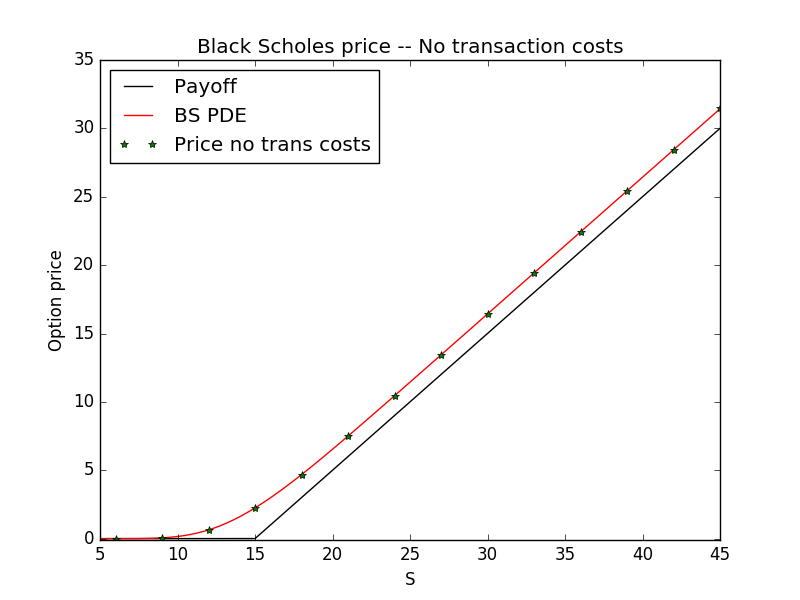
\includegraphics[width=\linewidth]{BS_No_costs.png}
   %\caption{Writer prices with zero transaction costs for diffusion process. Parameters are in the table \ref{tab:BS}.}
   %\label{Fig1} 
 \end{minipage}
 \ \hspace{2mm} \hspace{3mm} \
 \begin{minipage}[b]{0.5\linewidth}
  \centering
   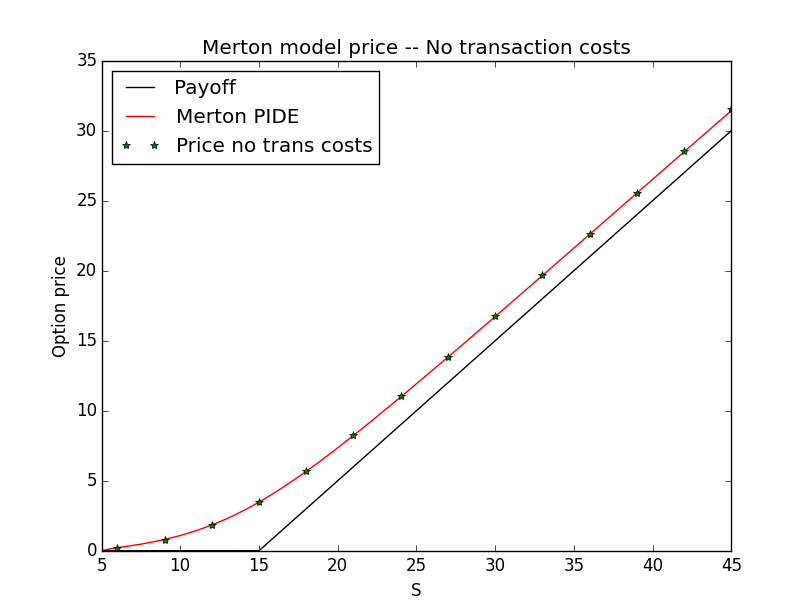
\includegraphics[width=\linewidth]{no_costs.png}
   %\caption{Writer prices with zero transaction costs for Merton process. Parameters are in the table \ref{tab:Mert}.}
   %\label{Fig2}
 \end{minipage}
  \ \hspace{2mm} \hspace{3mm} \
  \begin{minipage}[b]{\linewidth}
  \centering
   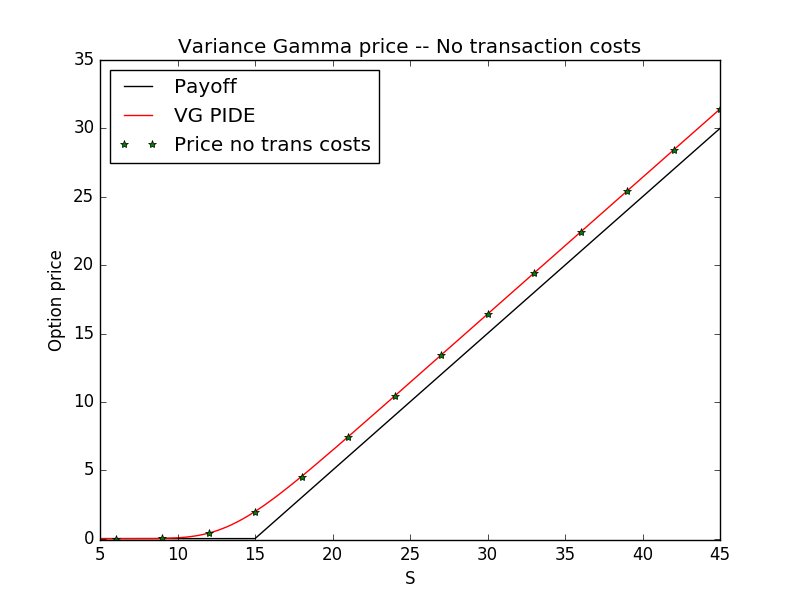
\includegraphics[width=0.51\linewidth]{No_costs_VG.png}
   \caption{Writer prices with zero transaction costs for diffusion (top-left), Merton (top-right) and VG (bottom) process. Parameters are in the Table \ref{tab:parameters}.}
   \label{Fig1}
 \end{minipage}
\end{figure}
We compute the option prices using the standard 
\emph{martingale pricing theory} presented in Chapter \ref{Chapter2}. In the Table \ref{tab:ATM_price} we show the \emph{at the money} values obtained with the closed formula 
and by solving the respective PIDE (see Table \ref{tab:prices_BS_M_VG}). 
The PIDE prices are obtained by solving the equations (\ref{BS_PDE}), (\ref{Merton_PIDE}) and (\ref{VG_PIDE}).
Of course, the parameter $\mu$ has not been used to compute the prices in Tab. \ref{tab:ATM_price}. 
In Section (\ref{properties_model}), we prove with a numerical experiment that
even in the model with transaction costs, the drift $\mu$ does not play an important role for the option price.
In the following analysis, we consider the PIDE prices as our benchmarks for comparisons.   
In all the computations we use equal transaction costs for buying and selling, $\theta_b = \theta_s$.

%%%%%%%%%%%%%%%%%%%%%%%%%%%%%%%%%%%%%%%%%%%%%%%%%%%%%%%%%%%%%%%%%%%%%%%%


In Fig. \ref{Fig1} we show that model prices replicate the PIDE prices for zero transaction costs and small values of $\gamma$. 
The values of $\gamma$ in the Table \ref{tab:parameters},
are chosen very small\footnote{ In Chapter 5 of \cite{GK99} are presented some common values for the risk aversion coefficient: $\gamma=0.3$, $\gamma=0.2$ and $\gamma=0.1$ 
for high, medium and low level of risk aversion respectively.} for this purpose. 
An intuitive argument to justify this choice is that for $\gamma \to 0$, the utility function 
can be approximated by a linear utility $\mathcal{U}(w) = 1 - e^{-\gamma w} \approx \gamma w$ and the investor can be considered risk neutral. 
A rigorous argument can be found in \cite{BaSo98}, where the authors use asymptotic analysis for small values of $\theta_b$, $\theta_s$ and $\gamma$ to derive 
a nonlinear PDE for the option price. For zero transaction costs this equation corresponds to the Black-Scholes PDE. 
Their argument can be extended also to PIDEs.
% \begin{figure}[t!]
%  \begin{minipage}[b]{0.5\linewidth}
%    \centering
%    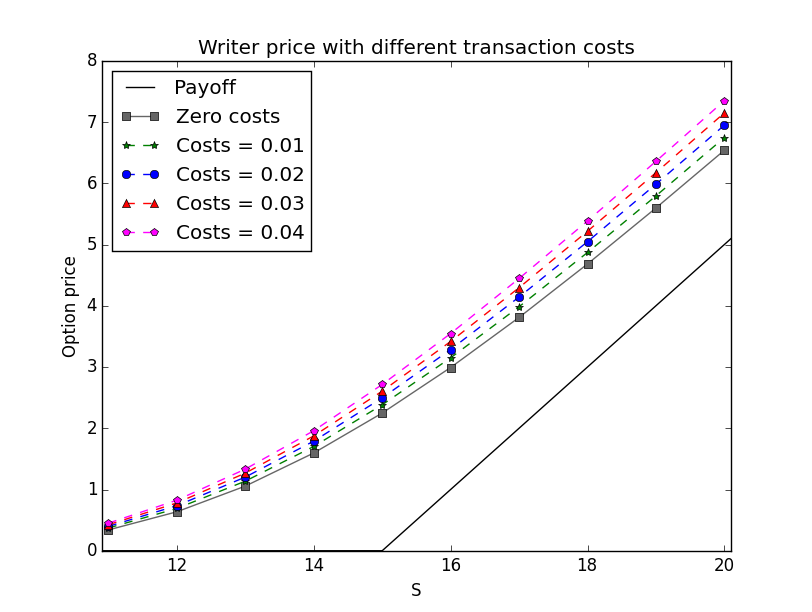
\includegraphics[width=\linewidth]{Trinomial_writer.png}
% %   \caption{Writer prices for different transaction costs. The continuous line is the solution of the Black-Scholes PDE.}
% %   \label{Fig4} 
%  \end{minipage}
%  \ \hspace{2mm} \hspace{3mm} \
%  \begin{minipage}[b]{0.5\linewidth}
%   \centering
%    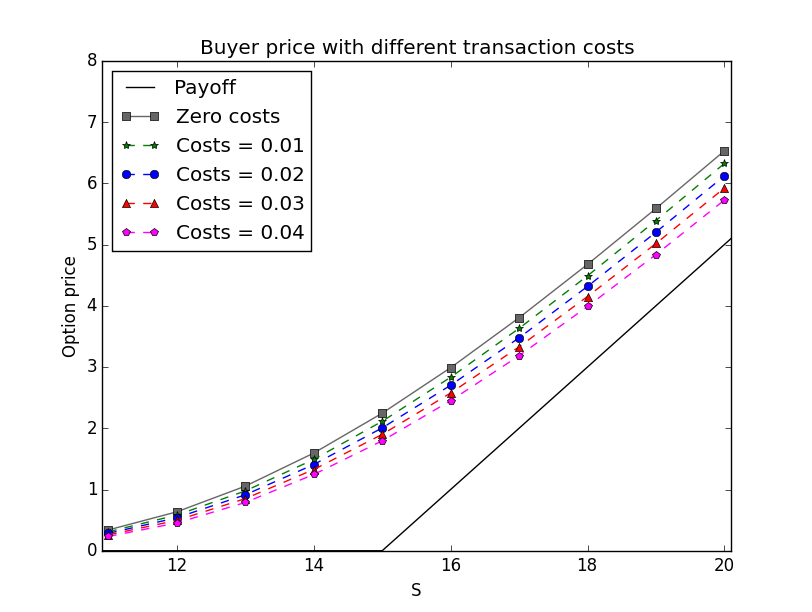
\includegraphics[width=\linewidth]{Trinomial_buyer.png}
%  \end{minipage}
%     \caption{Writer and buyer prices for different levels of transaction costs. The continuous line is the solution of the Black-Scholes PDE.}
%    \label{Fig2}
% \end{figure}
\begin{figure}[t!]
   \centering
   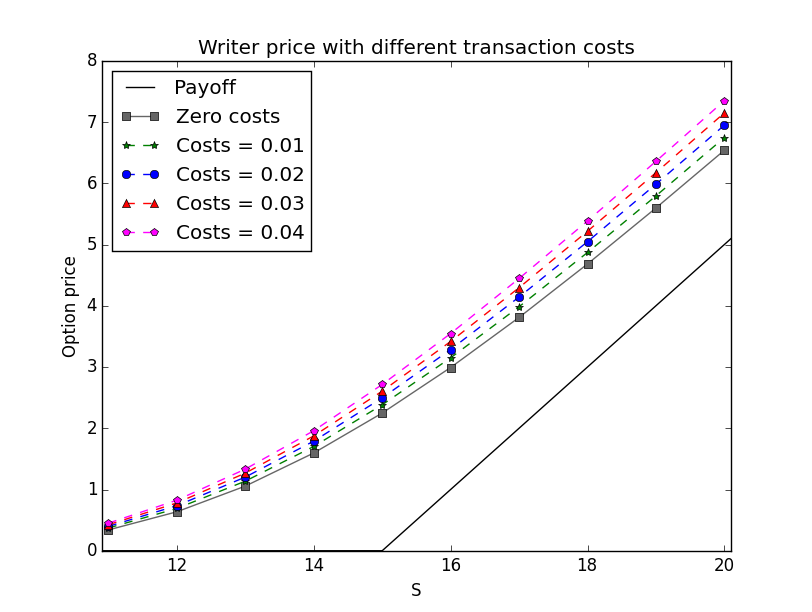
\includegraphics[scale=0.5]{Trinomial_writer.png}
   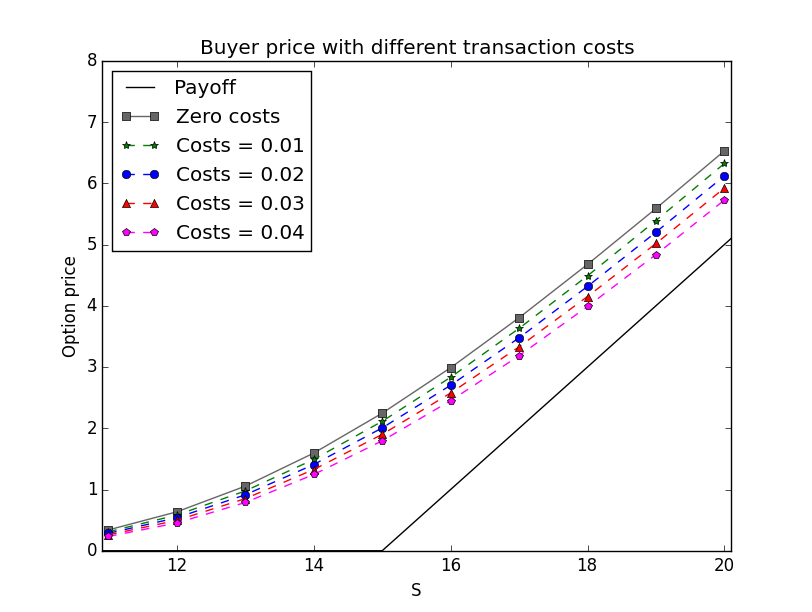
\includegraphics[scale=0.5]{Trinomial_buyer.png}
    \caption{Writer and buyer prices for different levels of transaction costs. The continuous line is the solution of the Black-Scholes PDE.}
   \label{Fig2}
\end{figure}

\begin{table}[ht]
\centering
 \begin{tabular}{*{11}l}
 \toprule
  \multicolumn{5}{c}{\textbf{Convergence table}} \\
  \midrule
  $N = \bar M$ & $\gamma = 0.0001$ & $\gamma = 0.001$ & $\gamma = 0.01$ & Execution time \\
  \midrule
    50   & 2.241214 & 2.241764 & 2.247311 & 0.01 $\pm$ 0.004\\
    100  & 2.249142 & 2.249506 & 2.253159 & 0.02 $\pm$ 0.005\\
    200  & 2.245422 & 2.245676 & 2.248216 & 0.11 $\pm$ 0.02\\
    400  & 2.246784 & 2.246959 & 2.248717 & 0.85 $\pm$ 0.04 \\
    800  & 2.246288 & 2.246271 & 2.247635 & 8.63 $\pm$ 0.1 \\
    1600 & 2.246576 & 2.246662 & 2.247515 & 82.44 $\pm$ 2.71\\
    3200 & 2.246412 & 2.246471 & 2.247068 & 910.8 $\pm$ 10.5\\
    3500 & 2.246366 & 2.246423 & 2.246993 & 1291.3 $\pm$ 13\\
  \bottomrule
  \end{tabular}
  \caption{Convergence table for ATM diffusion prices with zero transaction costs.}
  \label{tab:convergence}
\end{table}

\subsection{Diffusion results}

In the Figure \ref{Fig2} we show the diffusion writer and buyer prices with different
transaction costs.  
We can see that a higher transaction cost corresponds to a higher writer price, while a lower transaction cost corresponds to a lower buyer price.
In fact, the writer and buyer prices are respectively increasing and decreasing functions of the transaction cost, as already verified in \cite{ClHo97}.
The prices Figures \ref{Fig2}, are calculated with $N=1500$ time steps and $\bar M = N$. 
In the Table \ref{tab:convergence} we show ATM option prices for different values of $N$, with $\theta_s = \theta_b = 0$ and different risk aversion coefficients.
For $\gamma=0.0001$ and $N=3500$ the price is identical, up to the fourth decimal digit, to the original Black-Scholes price in Table \ref{tab:ATM_price}. 
Using the values in the Table \ref{tab:convergence} it is possible to perform a \emph{numerical convergence analysis} (see Section \ref{num_conv_analysis}).
We also present the execution times, from which we can estimate the asymptotic \emph{time complexity} of the algorithm. 
In Section (\ref{algorithm_Sect}) we estimated a complexity of $\mathcal{O}(N^{4})$. From the Table \ref{tab:convergence}, 
we obtain the exponent $\frac{\log(1291.3/910.8)}{\log(3500/3200)} = 3.9$, which is very close to the predicted value.  
The algorithm is written in Matlab using vectorized operations, and runs on an Intel i7 (7th Gen) with Linux.

\subsection{Merton results}

\begin{figure}[t!]
   \centering
   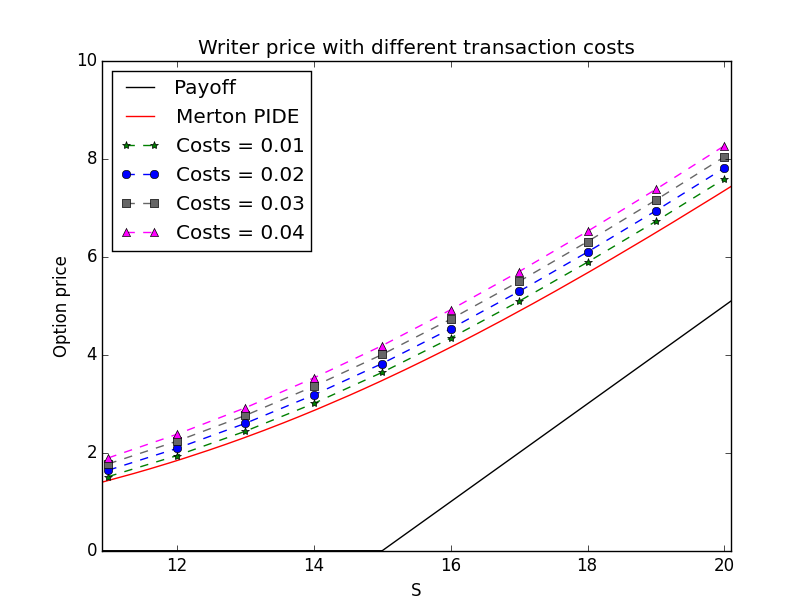
\includegraphics[scale=0.5]{writer_cost.png}
   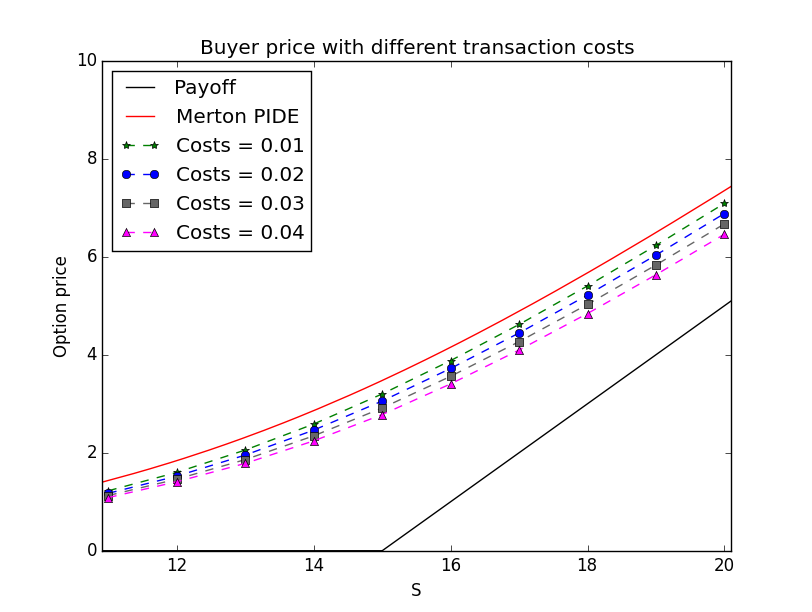
\includegraphics[scale=0.5]{Price_buyer.png}
   \caption{Writer and buyer prices for different transaction costs. The continuous line is the solution of the Merton PIDE.}
   \label{Fig3}
\end{figure}
In the Figure \ref{Fig3} we show the writer and buyer prices for the Merton process, with parameters in Tab. \ref{tab:parameters}.
An interesting feature of the multinomial tree construction for jump-diffusion processes is that $\bar L \propto \sqrt{N}$.
The integral domain is restricted to the bounded domain $[-B_1,B_2]$ with length $B_1+B_2 = \bar L \, h_x$. 
We choose the size of a space step $h_x = \sqrt{\E[\Delta X^2]} = \sigma_X \sqrt{\Delta t}$ and $\sigma_X^2 = \sigma^2 + \tilde \sigma_J^2$ 
with $ \tilde \sigma_J^2 = \int_{-B_1}^{B_2} z^2 \nu(dz)$.
However, the size of the Poisson jumps does not scale with $\Delta t$. So the number $\bar L$ has to be chosen big enough in order 
to have $L\, h_x \geq B_1+B_2$. 

In general, for a fixed $h_x$, the interval $[-B_1,B_2]$ should be chosen as big as possible. In practice, the choice of the truncation depends on the shape of the L\'evy measure.  
The Figures \ref{Fig13}, \ref{Fig14} show two examples with $[-B_1,B_2] = [\sqrt{\lambda} \xi,\sqrt{\lambda} \xi]$ and $[-B_1,B_2] = [-3\sqrt{\lambda} \xi,3\sqrt{\lambda} \xi]$ 
respectively. These choices correspond to 
$\bar L = 17$ and $\bar L = 52$.
For the Merton L\'evy measure (a scaled Normal distribution), a good choice is $[-B_1,B_2] = [-3\sigma_J,3\sigma_J]$, where  
$\sigma_J^2 = \int_{\R} z^2 \nu(dz) = \lambda(\alpha^2 + \xi^2)$ is the variance of the jump component of the Merton process.
The length of the interval is $\bar L \, h_x = 6\sigma_J$. 
It is well known that the integral over this region is about the $99.74\%$ of the total area.      
Using this interval and the parameters in Tab. \ref{tab:parameters} we obtain the relation $\bar L \geq 5.86 \sqrt{N}$.
In the calculation of the Merton prices in Fig. \ref{Fig3}, we used a discretization with $N=\bar M =100$, and $\bar L = 81$, 
with a good balance between small computational time and small price error. 
\begin{figure}[t!]
   \centering
   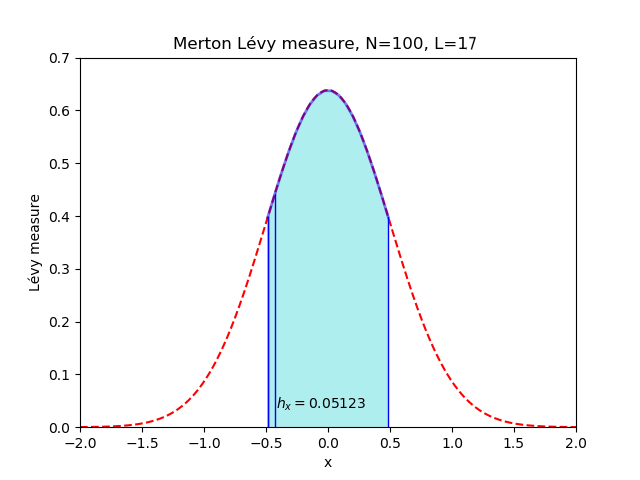
\includegraphics[scale=0.6]{Mert61_31.png}
   \caption{Merton L\'evy measure computed using parameters in Tab. \ref{tab:parameters}, $N=100$ and $\bar L=17$. 
   The domain $[-B_1,B_2] = [-\sqrt{\lambda} \xi,\sqrt{\lambda} \xi]$ has length $\bar L h_x \approx 2 \sqrt{\lambda} \xi$.}
   \label{Fig13} 
\end{figure}
\begin{figure}[t!]
   \centering
   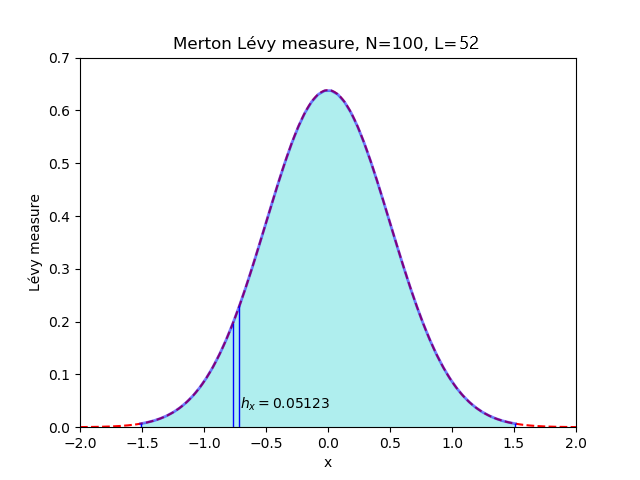
\includegraphics[scale=0.6]{Mert101_31.png}
   \caption{Merton L\'evy measure computed using parameters in Tab. \ref{tab:parameters}, $N=100$ and $\bar L=52$. 
   The domain $[-B_1,B_2] = [-3\sqrt{\lambda}\xi,3\sqrt{\lambda}\xi]$ has length $\bar L h_x \approx 6 \sqrt{\lambda} \xi$.}
   \label{Fig14}
\end{figure}

The convergence Tab. \ref{tab:convergence2} shows different Merton prices for different values of $N$ and $\bar L$.
Looking at the table from left to right, for each fixed $N$ it is possible to note how the truncation error decreases when $\bar L$ increases.
\begin{table}[ht]
\centering
 \begin{tabular}{*{6}l}
 \toprule
  \multicolumn{6}{c}{\textbf{Truncation error table}} \\
  \midrule
  $N$ & $\bar L=51$ &   $\bar L=71$   & $\bar L=91$ & $\bar L=101$ & $\bar L=111$ \\
  \midrule
    50   & 3.481318 & 3.481616 & 3.481617 & 3.481617 & 3.481617  \\
    100  & 3.468774 & 3.478806 & 3.479141 & 3.479146 & 3.479146  \\
    150  & 3.439090 & 3.474403 & 3.477574 & 3.477714 & 3.477742  \\
    200  & 3.399442 & 3.466338 & 3.476439 & 3.477234 & 3.477457 \\
  \bottomrule
  \end{tabular}
  \caption{Truncation error for ATM Merton prices with zero transaction costs.}
  \label{tab:convergence2}
\end{table}

\begin{table}[ht]
\centering
 \begin{tabular}{llll}
 \toprule
  \multicolumn{4}{c}{\textbf{Convergence table}} \\
  \midrule
  $N = \bar M$ & $\bar L$ & Price & Execution time \\
  \midrule
    50  & 61  & 3.481600 & 2.20 $\pm$ 0.08 \\
    75  & 75  & 3.479980 & 15.15 $\pm$ 0.07 \\
    100 & 91  & 3.479141 & 63.04 $\pm$ 0.49 \\
    125 & 97  & 3.478254 & 148.4 $\pm$ 1.16 \\
    150 & 105 & 3.477731 & 315.3 $\pm$ 5.58 \\
    175 & 113 & 3.477610 & 585.7 $\pm$ 10.57 \\ 
    200 & 121 & 3.477513 & 1106.0 $\pm$ 12.2 \\
  \bottomrule
  \end{tabular}
  \caption{Convergence table for ATM Merton prices with zero transaction costs.}
  \label{tab:convergence3}
\end{table}


In Table \ref{tab:convergence3} we show several prices with increasing values of $N$ and $\bar L$. We choose $\bar L$ big enough, such that the truncation error can be ignored.
Given the high computational complexity of the algorithm, 
it is difficult to present prices with bigger values of $N$,$\bar L$. For larger values of $N$ and smaller $\gamma$, we expect a convergence to the Merton price in Tab. 
\ref{tab:ATM_price}. 
The computational complexity in this case is expected to be $\mathcal{O}(N^{4.5})$. From the Table \ref{tab:convergence3} we get 
the exponent equal to $\frac{\log(1106.0/585.7)}{\log(200/175)} = 4.76$. Considering the errors, the results is not so different from the predicted value.

\subsection{VG results}\label{num_sec_VG}

\begin{figure}[t!]
   \centering
   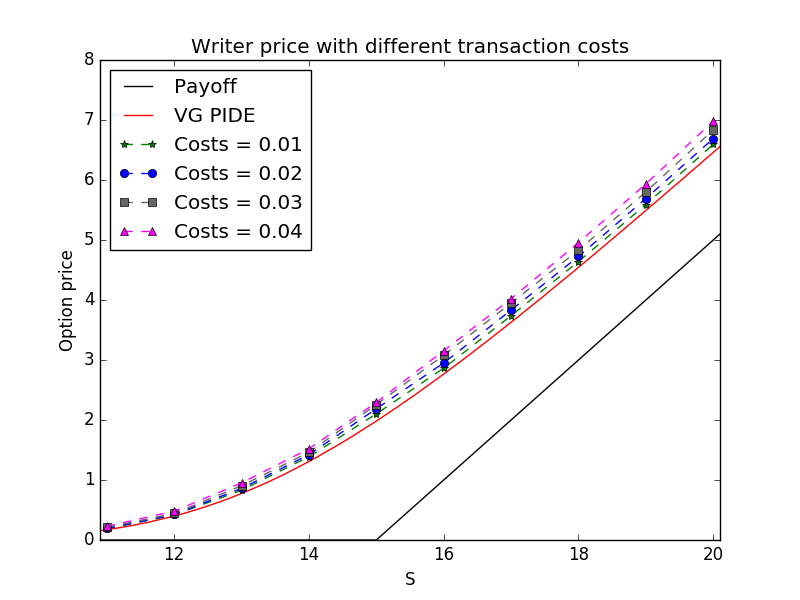
\includegraphics[scale=0.5]{VG_Writer.png}
   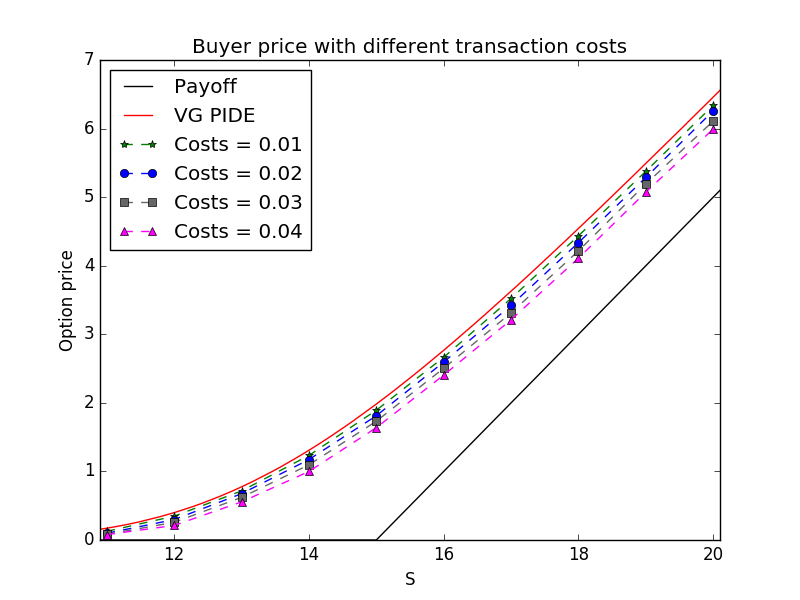
\includegraphics[scale=0.5]{VG_Buyer.png}
 \caption{Writer and buyer prices for different transaction costs. The continuous line is the solution of the VG PIDE.}
 \label{Fig8}
\end{figure}  

In the Figure \ref{Fig8} we show how the writer and buyer prices for the VG process change for several level of transaction costs (parameters in Tab. \ref{tab:parameters}). 
In these computations we used $N=\bar M = 150$ and $\bar L = 43$, such that the program can run in a reasonable computational time. 
The integration region in \ref{VG_inf_gen} is restricted to $[-B_1,-\epsilon]\bigcup [\epsilon,B_2]$ with $\epsilon=1.5h_x$. The choice of $B_1$ and $B_2$ depends on the shape of the 
L\'evy measure. 
In Fig. \ref{Fig15} and \ref{Fig16} we show two examples for the VG L\'evy measure (using parameters in Table \ref{tab:parameters}) with $N=150$, $h_x=0.0165$ and $N=1000$, $h_x=0.0064$. 
The two L\'evy measures are normalized, such that the integral on the region $[-\infty,-\epsilon]\bigcup [\epsilon,+\infty]$ is equal to one. The 
area underlying the functions on $[-B_1,-\epsilon]\bigcup [\epsilon,B_2]$ is highlighted for clarity.
For $\bar L = 43$, we can see that in both cases it is possible to cover a very high percentage of the initial unrestricted region. We can conclude that, unlike the Merton
measure, we do not need a big truncation interval.
Given the space step $h_X = \sigma_X\sqrt{\Delta t}$, with  
$ \sigma_X^2 = \hat \sigma_{J}^2 + \sigma_{\epsilon}^2 $ and $\hat \sigma_J^2 = \int_{[-B_1,-\epsilon]\bigcup [\epsilon,B_2]} z^2 \nu(dz)$, 
it is enough to consider a region at least as big as the standard deviation  
of the unrestricted jump process\footnote{For small values of $\epsilon$ the value of $\sigma_{\epsilon}^2$ is negligible. In this case it is possible to use the expression for the 
variance of the VG process and write $\sigma_X^2 = \bar \sigma^2 + \theta^2 \kappa$.}
i.e. $h_X \bar L \geq \sigma_J$, where $\sigma_J^2 = \int_{[-\infty,-\epsilon]\bigcup [\epsilon,\infty]} z^2 \nu(dz)$. 
Putting all together, the relation becomes $\bar L\geq \frac{\sigma_J}{\sigma_X} \sqrt{N}$, and replacing the values $\sigma_X = 0.2024$ and $\sigma_J=0.1916$ 
we get $\bar L \geq 0.94 \sqrt{N}$.
\begin{figure}[t!]
   \centering
   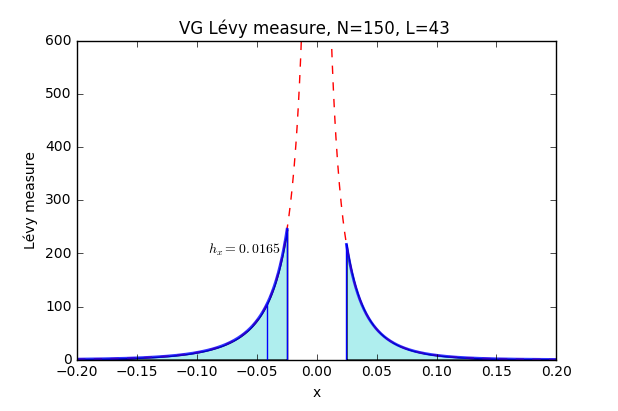
\includegraphics[scale=0.6]{VG43.png}
   \caption{VG L\'evy measure computed using parameters in Tab. \ref{tab:parameters}, $N=150$ and $\bar L=43$. 
   The domain $[-B_1,-\epsilon]\bigcup [\epsilon,B_2]$ has length $(\bar L-3) h_x$. The highlighted area is $99.9\%$ of the total area.}
   \label{Fig15} 
\end{figure}
\begin{figure}[t!]
  \centering
   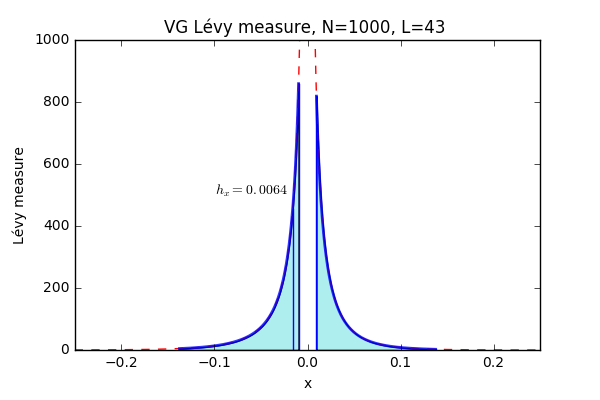
\includegraphics[scale=0.6]{VG1000.png}
   \caption{VG L\'evy measure computed using parameters in Tab. \ref{tab:parameters}, $N=1000$ and $\bar L=43$. 
   The domain $[-B_1,-\epsilon]\bigcup [\epsilon,B_2]$ has length $(\bar L-3) h_x$. The highlighted area is $98.9\%$ of the total area.}
   \label{Fig16}
\end{figure}

In the Table \ref{tab:convergence4} we present several option prices computed with different values of $N$, but with fixed $\bar L$.
In the case of the VG process it is more difficult to analyze the convergence results.
This is due to the approximation (\ref{log_sde_inf_act2}) introduced to replace the infinite activity jump component with a Brownian motion. All the parameters
in (\ref{sig_eps}) depend on $\epsilon$, and consequently on $N$.
Within our discretization ($N=150$), we have $\sigma_{\epsilon} = 0.0654$, $\lambda_{\epsilon} = 10.01$. 
With the parameters under consideration, we obtain an ATM price for zero transaction costs of 1.9821, which is very close the the PIDE price in Tab. \ref{tab:ATM_price}. 

The convergence rate of the VG PIDE is quite low and this is reflected in our algorithm. We refer to \cite{CoVo05b} for a detailed error analysis.
In order to solve the PIDE (using an implicit-explicit scheme) we constructed
a grid with 13000 space steps of size $\delta x = 0.0004$ and 7000 time steps, and obtained the price in Tab \ref{tab:ATM_price}, 
with an approximated activity $\lambda_{\epsilon} = 75$.
Consequently, we expect to have good convergence results in our algorithm when $N\sim 10^4$.
All the presented prices (Figures \ref{Fig8}) have thus a truncation error, which is adjusted by an accurate choice of the value of $\gamma$. 
\begin{table}[ht]
\centering
 \begin{tabular}{llll}
 \toprule
  \multicolumn{4}{c}{\textbf{Convergence table}} \\
  \midrule
  $N = \bar M$ & $\lambda_{\epsilon}$ & Price & Execution time \\
  \midrule
    50  & 4.73  & 1.910934 & 3.63 $\pm$ 0.16 \\
    100 & 7.82  & 1.957806 & 26.54 $\pm$ 0.26 \\
    150 & 10.01 & 1.982078 & 82.51 $\pm$ 0.20 \\
    200 & 11.73 & 1.996180 & 185.2 $\pm$ 0.81 \\
    250 & 13.14 & 2.004719 & 350.3 $\pm$ 4.5 \\
    300 & 14.35 & 2.008536 & 654.2 $\pm$ 7.3\\ 
    350 & 15.40 & 2.009436 & 1236 $\pm$ 12 \\
  \bottomrule
  \end{tabular}
  \caption{Convergence of ATM VG prices with $\bar L =43$, zero transaction costs.}
  \label{tab:convergence4}
\end{table}

From Tab. \ref{tab:convergence4} we can estimate the time complexity of this algorithm. The exponent is $\frac{\log(1236.0/654.2)}{\log(350/300)} = 4.12$, 
indeed very close to the theoretical $\mathcal{O}(N^4)$. 


\subsection{Numerical convergence analysis}\label{num_conv_analysis}

In this section we want to analyze the convergence properties of the Algorithm [\ref{algo}] considering the prices presented in 
Tables \ref{tab:convergence}, \ref{tab:convergence3} and \ref{tab:convergence4}. 

\begin{figure}[t!]
 \begin{minipage}[b]{0.5\linewidth}
   \centering
   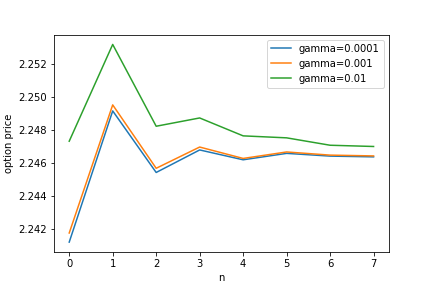
\includegraphics[width=\linewidth]{diff_1.png}
   \caption{Prices in table \ref{tab:convergence} as function of $n=\log_2(N/50)$.}
   \label{Fig_err1} 
 \end{minipage}
  \
  \begin{minipage}[b]{0.5\linewidth}
  \centering
   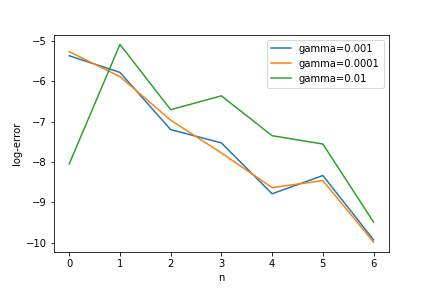
\includegraphics[width=\linewidth]{diff_3.png}
   \caption{Plot of the log-errors as function of $n=\log_2(N/50)$.}
   \label{Fig_err3}
 \end{minipage}
 \
  \begin{minipage}[b]{0.5\linewidth}
   \centering
   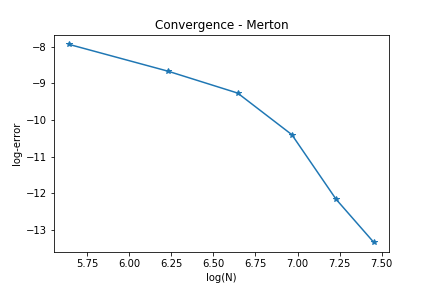
\includegraphics[width=\linewidth]{Mert_1.png}
   \caption{Plot of the log-errors as function of $n=\log_2(N/50)$, for Merton prices in \ref{tab:convergence3}}
   \label{Fig_err4} 
 \end{minipage}
 \
 \begin{minipage}[b]{0.5\linewidth}
  %\centering
   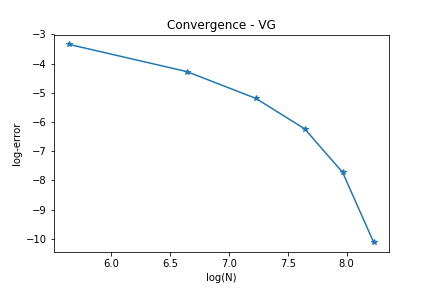
\includegraphics[width=\linewidth]{VG_1.png}
   \caption{Plot of the log-errors as function of $n=\log_2(N/50)$, for VG prices in \ref{tab:convergence4}}
   \label{Fig_err5}
 \end{minipage}
\end{figure} 

Let us first consider the prices in Table \ref{tab:convergence}, which are plotted in Figure \ref{Fig_err1}. 
We can see that for higher values of $\gamma$, not only the price increases, but the oscillations of the log-error increases as well.
Let us assume the limit price $V^*$ is represented by the price at $N=3500$. 
For computational reasons, i.e. the very high computational time, it was not possible to consider higher values. 
Following the arguments in Section \ref{numerical_concergence_section}, let us define the log-error $\log_2 (\varepsilon_N)$ with $\varepsilon_N = |V^N - V^*|$. 
Then we consider $n = 0,1,...,6$ such that $N = 50\cdot2^n$.
In Figure \ref{Fig_err3} we plot the log-error for each value of $n$.
For $\gamma=0.0001$ and $\gamma=0.001$, even if the line is not straight, it is possible to recognize a linear behavior.  
In these cases it is possible to estimate the rate of convergence (the slope of the line is about $-1$ i.e. linear convergence).  
For $\gamma=0.01$, given the irregular shape, it is hard to understand the functional behavior. 
The value at $n=0$ can be excluded because it is probably an outlier originated by the rough grid resolution.
In general, given the nonlinear nature of the optimization problem, we expect a nonlinear behavior of the convergence functional form.

This is confirmed by the Pictures \ref{Fig_err4} and \ref{Fig_err5}, 
containing the prices obtained for the jump-diffusion Merton process in Table \ref{tab:convergence3}, and the VG process in Table \ref{tab:convergence4}.
The shape is more regular (here the number of steps $N$ is much smaller), but it is not a linear function. 
The algorithm converges faster for higher values of $N$.



\subsection{Properties of the model}\label{properties_model}

\begin{table}[ht]
  \centering
 \begin{tabular}{llllll}
\toprule
 & cost = 0 & cost = 0.01 & cost = 0.02 & cost = 0.03 & cost = 0.04  \\
\midrule
\textbf{Merton} & 3.4771 & 3.6400 & 3.8212 & 4.0054 & 4.1864 \\
\textbf{VG} & 1.9821 & 2.0921 & 2.1870 & 2.2568 & 2.3131 \\
\bottomrule
\end{tabular}
  \caption{Merton and VG writer prices for different transaction costs, with parameters as in Tab. (\ref{tab:parameters}). }
  \label{tab:costs}
\end{table}

In this section we want to analyze the properties of the model and how the option price depends on the level of transaction costs $\theta_b$, $\theta_s$, 
the risk aversion parameter $\gamma$ and the drift $\mu$. 
In this numerical experiment, we use the Merton model with parameters of Tab. \ref{tab:parameters}.
In Tab. \ref{tab:costs} we show the writer ATM option values for different transaction costs.  
\begin{figure}[t!]
 \begin{minipage}[b]{0.5\linewidth}
   \centering
   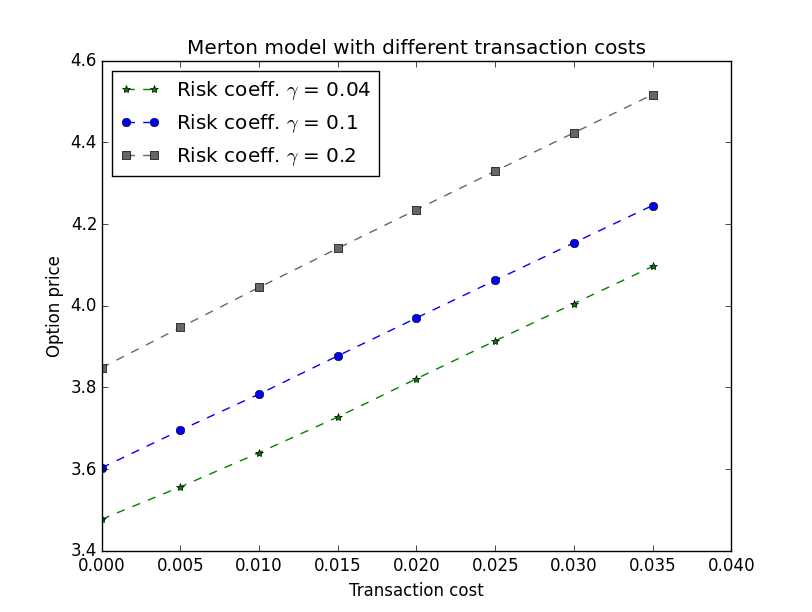
\includegraphics[width=\linewidth]{P_vs_cost.png}
   \caption{Merton option prices for the writer as function of the transaction cost, with different values of $\gamma$.}
   \label{Fig10} 
 \end{minipage}
 \ \hspace{2mm} \hspace{3mm} \
 \begin{minipage}[b]{0.5\linewidth}
  \centering
   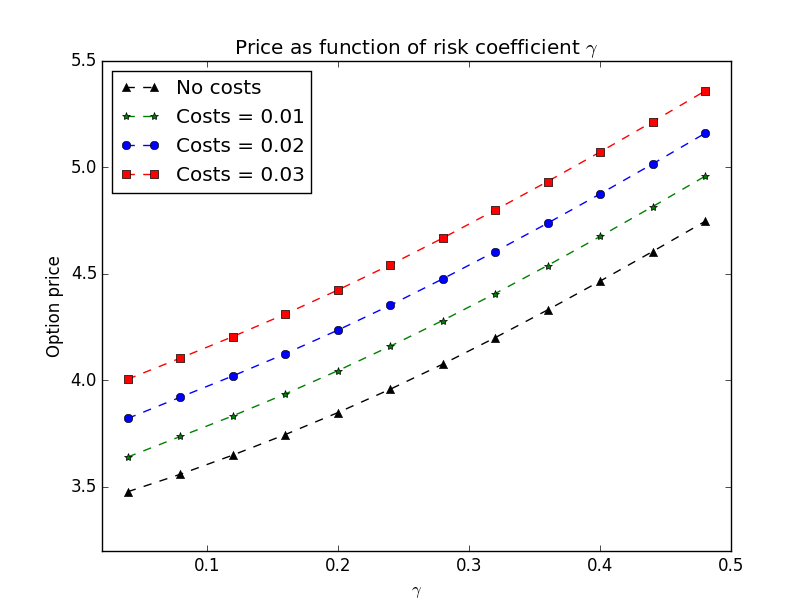
\includegraphics[width=\linewidth]{price_gamma.png}
   \caption{Merton option prices for the writer as function of $\gamma$, with different values of transaction costs.}
   \label{Fig11}
 \end{minipage}
  \ \hspace{2mm} \hspace{3mm} \
  \begin{minipage}[b]{\linewidth}
  \centering
   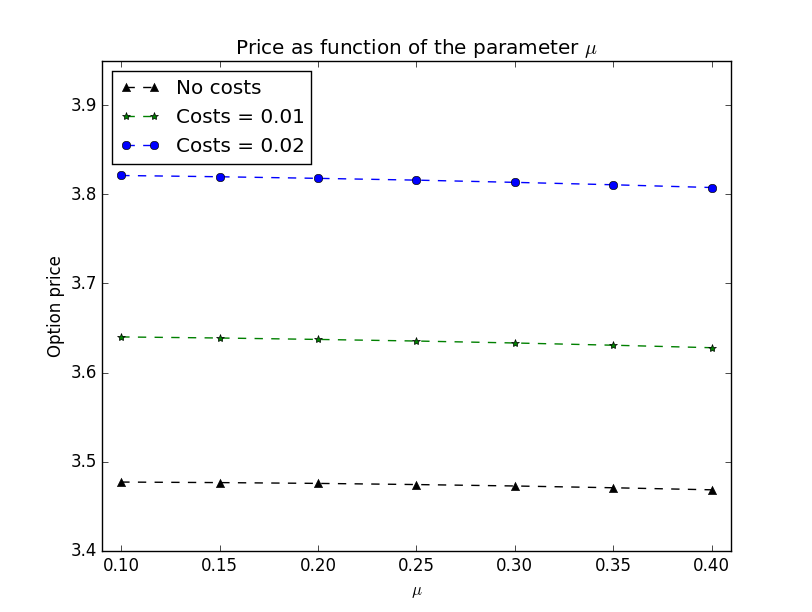
\includegraphics[width=0.55\linewidth]{price_mu2.png}
   \caption{Merton option prices for the writer as function of $\mu$, with different values of transaction costs.}
   \label{Fig12}
 \end{minipage}
\end{figure}


In Fig. \ref{Fig10} we can see better how the price for the writer is affected by the change of the transaction costs. 
The picture shows prices for different values of risk coefficient.
The risk profile of the investor also plays an important role. As already shown in \cite{HoNe89}, the writer price is an
increasing function of the risk aversion coefficient. Figure \ref{Fig11} confirms their results.

In all the previous computations we always used the drift term $\mu$ equal to the risk free interest rate $r$. This is the choice   
made in \cite{HoNe89}, following the common rule of the standard no-arbitrage
theory.
The option price has to be independent of the expected return of the underlying asset.
As we can see in Fig. \ref{Fig12}, the numerical experiment shows that also in this model, the option prices 
do not depend on the drift $\mu$.



\section{Solution of the 4-dimensional problem}\label{full_eq_section}

This section focuses on the original HJB equation \ref{HJB1}, were no variables reduction is considered. 
A few authors have already presented some results for the diffusion case, using different approaches.
In \cite{Pal15} the authors propose a method to improve the performances of the Markov chain approximation method for the diffusion case. In \cite{Song14} the author propose
a penalty method for the diffusion case of the 4 dimensional HJB equation, but the numerical results they present are not very clear.

If we want to solve the problem (\ref{max_probl1}), we have to deal with a three dimensional state. In the variable reduction Section \ref{variable_reduction}
we assumed a high value of credit availability $C$, such that the default probability can be ignored. 
Here we do not ignore the default case, and compute option prices for an investor with low credit availability.
We work with the original problem (\ref{max_probl1}) and derive a discrete time dynamic programming equation as done for (\ref{HJB3}).

Let us indicate with $B_n := B(t^-_n)$ the value of cash immediately before the possible transaction.
Let us define $\Sigma_b := \{-K_5 h_b , ... , -h_b,0,h_b, ... , +K_6 h_b \}$,  
where $h_b>0$ is the discrete cash step and  $K_5,K_6 \in \N$. Its dimension is $\bar B = \#(\Sigma_b) = K_5+K_6+1$.
The discretized SDE for the cash account process $\{B_t\}_{t \in [t_0,T]}$ in (\ref{porfolio_dynamics}), with solution (\ref{BT}), is:
\begin{equation}\label{Bn}
 B_{n+1} =  e^{r \Delta t} \biggl( B_n - (1+\theta_b) e^{X_n} \Delta L_n + (1-\theta_s) e^{X_n} \Delta M_n \biggr)
\end{equation}
Let us derive the backward algorithm for computing the value function using the DPP, as we did for (\ref{HJB3}). %The integral representation of \ref{HJB1} is:
We obtain the discrete DPE: 
\begin{align}\label{HJB5}
 & V(t_n,B_n,Y_n,X_n) = \max \; \biggl\{ \E_n 
 \biggl[ V \bigl( t_{n+1}, e^{r \Delta t} B_n, Y_n, X_n + \Delta X_n \bigr) \biggr], \\ \nonumber
 & \max_{\Delta L_n} 
 \E_n \biggl[ V \bigl( t_{n+1}, e^{r\Delta t}(B_n - e^{X_n}(1+\sigma_b)\Delta L_n) , Y_n + \Delta L_n, X_n + \Delta X_n \bigr) \biggr] , \\ \nonumber
 & \max_{\Delta M_n}
 \E_n \biggl[ V \bigl( t_{n+1}, e^{r\Delta t}(B_n + e^{X_n}(1-\sigma_s)\Delta M_n) , Y_n - \Delta M_n, X_n + \Delta X_n \bigr) \biggr]
 \biggr\},
\end{align}
where all the expectations are conditioned on the current state $(B_n,Y_n,X_n)$.  We use the notation $V(t_n, b_h, y_j, x_i) = V^n_{h,j,i}$

Following the arguments in Section \ref{algorithm_Sect}, the computational complexity is 
$$\mathcal{O}\biggl( (N+1)\bigl[\frac{N(\bar L-1)}{2}+1 \bigr] \times \bar M \times \bar B \times \min\{\bar M, \bar B\} \biggr).$$
The term $\min\{\bar M, \bar B\}$ is the computational complexity of the minimum search. 
% $\sum_{n,h,j,i} \bigl( \# \varPi(t_n,b_h,y_j,x_i) \bigr)$
It is performed for each $(t_n, b_h,y_j,x_i)$ such that of all $l,m \in \N$:
$$ y_j+l h_y \in \Sigma_y \bigcap (b_h - e^{x_i}(1+\sigma_b)l h_y) \geq -K_5 h_b $$ 
and 
$$y_j-m h_y \in \Sigma_y \bigcap (b_h + e^{x_i}(1-\sigma_s)m h_y) \leq K_6 h_b .$$ 
If we set $\bar L = \sqrt{N}$ and $\bar B = \bar M = N$ we have total computational complexity $\mathcal{O}(N^{5.5})$. 

In the following analysis of the problem (\ref{max_probl1}), we assume that $\mathcal{U}(w) = -C$ for $w < -C$ and $\beta = r$. 
In Figure (\ref{Fig21}) it is possible to see the shape of the value function at terminal time for different values of $\gamma$.
In the points $(b,y,x)$ such that $\mathcal{W}(b,y,x) = -C$ the function is not differentiable, and this may create some instabilities in the numerical computations. 
%However this assumption will be useful in order to speed up the algorithm.

\begin{figure}[t!]
   \centering
   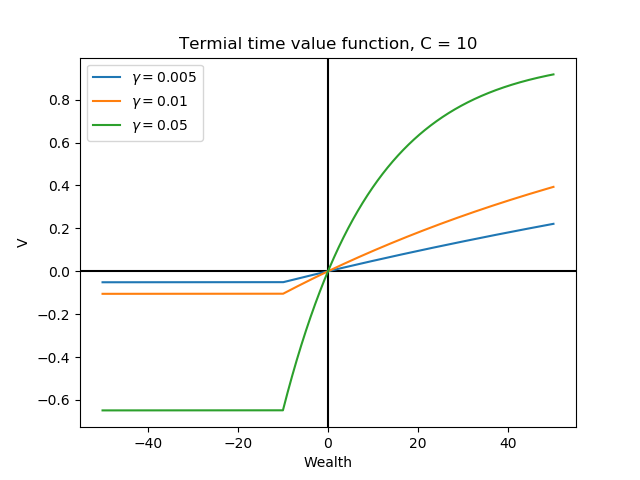
\includegraphics[width=0.7\linewidth]{terminal_utility.png}
   \caption{Terminal time value functions with $\mathcal{U}(w) = -C$ for $w < -C$.}
   \label{Fig21} 
\end{figure}
\begin{figure}[t!]
   \centering
   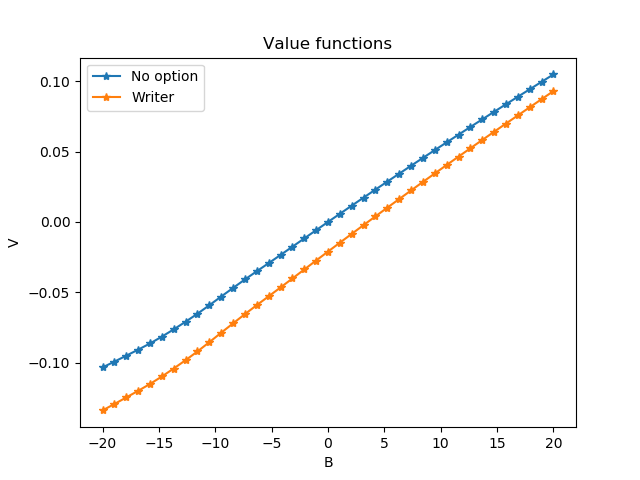
\includegraphics[width=0.6\linewidth]{value_f_C5000.png}
   \caption{Value function for the writer and value function with no option at time $t_0$ with $Y_0=0$ and $S_0=15$. Parameters in Tab. \ref{tab:parameters} and 
   $\theta_b = \theta_s = 0$. 
   The option price at $B_0=0$ is $p^w=3.48303858$.}
   \label{Fig22} 
\end{figure}

\begin{algorithm}[H] 
\caption{Backward algorithm}
\label{algo2}
 \algsetup{indent=1.5em}
 \begin{algorithmic}[1]
    \REQUIRE $r, (b,\sigma,\nu), X_0, K, T, \theta_b, \theta_s, \gamma, N, \bar L, \bar M, \bar B. $
    \ENSURE $V^j(t_0,b,y,X_0)$ for $j=0,w,b$
      \STATE Create the lattice for (\ref{log_sde_discr}) and (\ref{Bn}) with appropriate discrete steps $\Delta t, h_y, h_x, h_b$.
      \STATE Create the vector of probabilities $p_k$ as defined in \ref{pK}.  
      \STATE Use (\ref{terminal_conditions}) to initialize a $\bar B \times \bar M \times \bigl( N(\bar L-1)+1 \bigl)$ grid for $V^N_{h,j,i}$.  
      \FOR {n = N-1 to 0}
      \STATE $W_{h,j,i} = \sum_{k = -K_1}^{K_2} p_k \; V^{n+1}_{h,j,i+k}$
      \STATE Interpolate the value of $W$ in the points: \\
             - $W_1(n,h,j,i) \mbox{ at } (t_n, e^{r \Delta t} b_h, y_j, x_i)$.\\
             - $W_2(n,h,j,i,l)$ at $(t_n, e^{r\Delta t}(b_h - e^{x_i}(1+\sigma_b)l h_y), y_j+l h_y, x_i ) $ for each $l$.\\
             - $W_3(n,h,j,i,m)$ at $(t_n, e^{r\Delta t}(b_h + e^{x_i}(1-\sigma_s)m h_y), y_j-m h_y, x_i ) $ for each $m$. 
      \STATE $V^{n}_{h,j,i} = \max \biggl\{ W_1(n,h,j,i), \, \max_l W_2(n,h,j,i,l), \, \max_m W_3(n,h,j,i,m)  \biggr\}$ 
      \ENDFOR
  \end{algorithmic}
\end{algorithm} 

We present numerical solutions for a Merton process with values in Table \ref{tab:parameters}. 
The cash vector is chosen such that $-20 \leq B_0 \leq 20$, and consider values of $N = \bar M = \bar B = 25$ and $\bar L = 11$, 
but even with these small values, the algorithm takes about 2 hours to run. 
The algorithm is written in Python and runs on a Linux machine with a i7 processor. 
%In order to increase the speed of the program
%it is necessary to write the program in a low level language such as C or Fortran.


In the Figure \ref{Fig22} we computed the value functions and the option prices for $C= 5000$.
The value functions are smooth and, as expected, the option price (defined in (\ref{writer}) ) corresponding to the horizontal distance between the value functions,
is not affected too much by the initial wealth. 
The high value of the credit availability $C$ 
has to be intended as a low default probability. 
Under this setting, this problem corresponds to the reduced problem with 3 variables (where the probability of default is ignored). 
As expected, also the numerical results reproduce the results in Section \ref{numerical}. 
The option price at $B_0=0$ is $p^w=3.48303858$, which is very close to the corresponding value in table \ref{tab:costs}.

A different story happens when we choose a small credit availability. For example $C = 10$.\\ 
In Figure \ref{Fig23} we can see that the two value functions have the same value for $B_0 < -C$, because in this region the value function corresponds to the boundary conditions
(remember that we are considering $Y_0=0$). 
For higher values of $B_0$, the influence of the boundary conditions decreases and the value functions look like those in Figure \ref{Fig22}.
\begin{figure}[t!]
 \begin{minipage}[b]{0.5\linewidth}
   \centering
   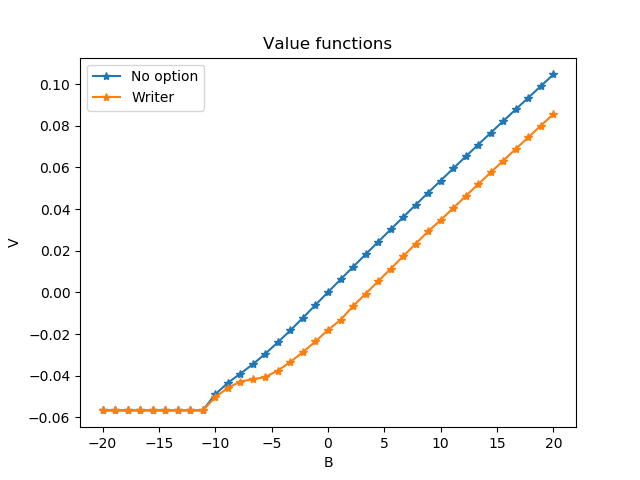
\includegraphics[width=\linewidth]{value_f_C10.png}
   \caption{Writer and no option value functions at $t_0$ with $C=10$, $Y_0=0$ and $S_0=15$.}
   \label{Fig23} 
 \end{minipage}
 \ \hspace{2mm} \hspace{3mm} \
 \begin{minipage}[b]{0.5\linewidth}
  %\centering
   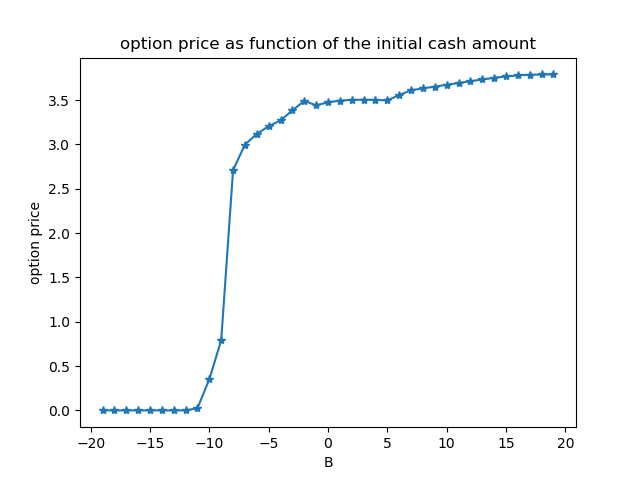
\includegraphics[width=\linewidth]{option_B.png}
   \caption{Option price as function of $B_0$ at $t_0$ with $C=10$, $Y_0=0$ and $S_0=15$.}
   \label{Fig24}
 \end{minipage}
\end{figure}  

It is important to stress that the grid resolution we used in these examples is quite low. 
Although we this algorithm is able to replicate quite well the results obtained in the previous sections,  
given its high complexity is not possible to study the convergence properties. 
Furthermore, the value function is highly non-linear. In the algorithm we used a linear interpolation to obtain the missing points in the grid, 
and this may create further errors when the discretization steps are large.

\begin{figure}[t!]
 \begin{minipage}[b]{0.5\linewidth}
   \centering
   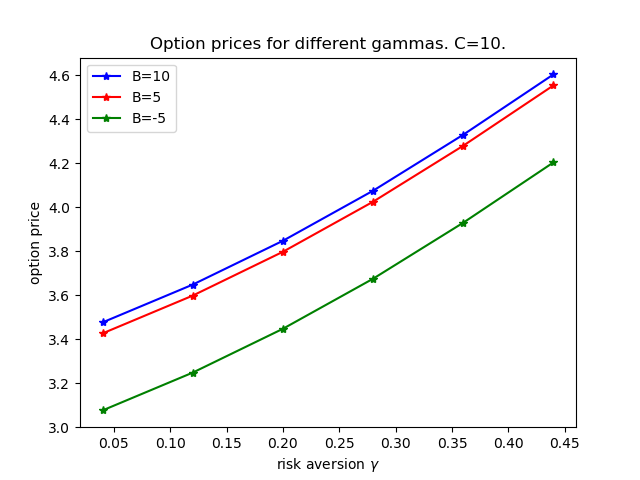
\includegraphics[width=\linewidth]{B_gamma_10.png}
   \caption{Option price as function of risk aversion, for several values of initial $B_0$. We set $C=10$, $Y_0=0$ and $S_0=15$.}
   \label{Fig26} 
 \end{minipage}
 \ \hspace{2mm} \hspace{3mm} \
 \begin{minipage}[b]{0.5\linewidth}
  %\centering
   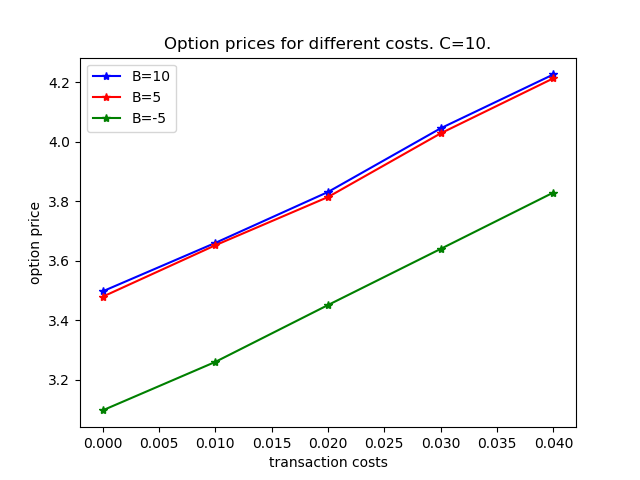
\includegraphics[width=\linewidth]{B_cost_10.png}
   \caption{Option price as function of transaction costs, for several values of initial $B_0$. We set $C=10$, $Y_0=0$ and $S_0=15$.}
   \label{Fig25}
 \end{minipage}
\end{figure}  

We conclude this section by testing the model properties as we did in Section \ref{properties_model}. 
In Figures \ref{Fig26} and \ref{Fig25} we present several values of option prices as function of the risk aversion and transaction costs respectively.  
We can see that the value of $B_0$ does not affect the shape of the curve, but only its height. 
As we saw in Figures \ref{Fig10} and \ref{Fig11}, the option price is an increasing function of the risk aversion and of the transaction costs.


\section{Multinomial method applied to the reduced problem}\label{multinomial_section}

In Section \ref{MC_section} we have seen that a possible technique to construct the Markov chain approximation is to discretize the infinitesimal generator
using an explicit finite difference scheme.
For Lévy processes with infinite activity, however, this technique cannot be used directly because of the singularity of the Lévy measure.
In Section \ref{VG_section2} we explained how to approximate the original process by a jump-diffusion process. 
The associated infinitesimal generator can be discretized using the same approach developed for jump-diffusion generators in Section \ref{Markov_Chain2}.
%However, in Section \ref{numerical_concergence_section}, we saw that the convergence of the (approximated) VG PIDE is very slow.

In this section, instead, we use the multinomial approximation method presented in Chapter \ref{Chapter3}.%, in place of the discretization proposed in Section \ref{Markov_Chain2}.
With this method the total computational complexity is reduced because the number of branches is kept fixed.
Although the method still relies on an approximation (the VG process is approximated by a general jump process with only the first four moments corresponding to the moments of the 
original VG process),
the number of branches is fixed to $\bar L = 5$, and therefore the computational complexity is reduced by a factor $\sqrt{N}$.
Recall that the complexity of the Algorithm [\ref{algo}] is 
$$\mathcal{O}\biggl( (N+1)\bigl[\frac{N(\bar L-1)}{2}+1 \bigr] \times \bar M \times \bar M \biggr).$$
Assuming $\bar M = N$ and $\bar L = 5$, the computational time is reduced to $\mathcal{O}(N^4)$. 
\begin{table}[t!]
%\begin{center}
%\begin{minipage}{0.5\linewidth}
\centering
 \begin{tabular}{||c|c||}
 \hline
  \multicolumn{2}{|c|}{Convergence table} \\
  \hline
  $N = \bar M$ & Price \\
  \hline
    50 & 1.96121076540 \\
  \hline
    100 & 1.96889900730 \\
  \hline  
    200 &  1.97154200723 \\
  \hline
    400 & 1.97288296067 \\
  \hline   
    800 & 1.97354995910  \\
  \hline
    1000 & 1.97368292970 \\ 
  \hline
    1600 & 1.97388226442  \\
  \hline
    2000 & 1.97394872091  \\  \hline
  \end{tabular}
  \caption{Convergence table for ATM VG prices with parameters in Tab. \ref{tab:parameters}, calculated with the multinomial method.}
  \label{tab:convergence31}
%\end{minipage}
\end{table}

\begin{figure}[t!]
% \begin{minipage}{0.5\linewidth}
  \centering
   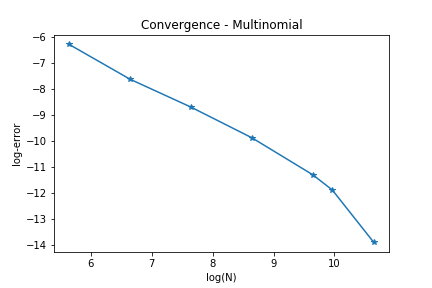
\includegraphics[scale=0.6]{Multinom_1.png}
   \caption{Multinomial VG writer and buyer prices for different transaction costs.}
   \label{Fig37}
% \end{minipage}
% \end{center}
\end{figure}  
In the numerical computations we used the VG parameters in Table \ref{tab:parameters}. 
The discretization scheme is implemented according to the method proposed in Chapter \ref{Chapter3} i.e. the space step has size given by Eq. (\ref{alphat}) and 
the transition probabilities are obtained by (\ref{probabilities2}). 
In Table \ref{tab:convergence31} we reported prices for different values of $N$.
Using these prices, in Figure \ref{Fig37} we plot the log-error as a function of the logarithm of $N$. We can see that there is a linear relation 
$\log_2(\varepsilon) \sim p \log_2(N)$ between them, with a rate of convergence $p$ which is about $p \approx 1.6$. 
In Figures \ref{Fig32} and \ref{Fig33} we present numerical results obtained using the multinomial method for different levels of transaction costs. 
\begin{figure}[t!]
% \begin{minipage}[b]{0.5\linewidth}
   \centering
   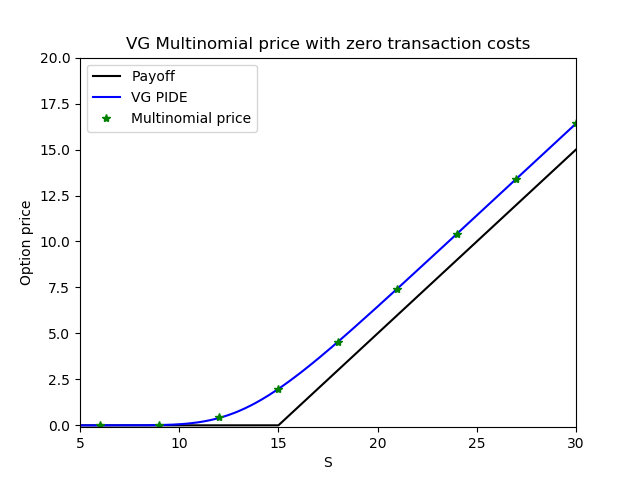
\includegraphics[scale=0.6]{Multi_VG_zerocosts.png}
   \caption{Comparison of multinomial VG prices with zero transaction costs and the solution of the VG PIDE (continuous line).}
   \label{Fig32} 
% \end{minipage}
\end{figure}
\begin{figure}[t!]
  \centering
   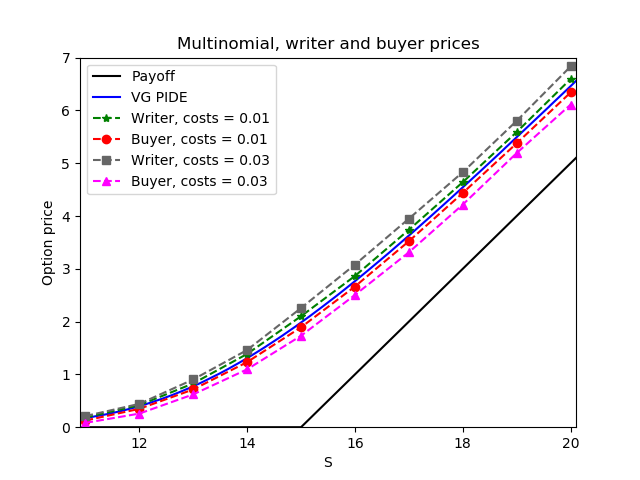
\includegraphics[scale=0.6]{Multi_VG_costs.png}
   \caption{Multinomial VG writer and buyer prices for different levels of transaction costs.}
   \label{Fig33}
\end{figure}  






\section{Chapter conclusions}


In Chapter \ref{Chapter5} we derived the general HJB equation of the model, eq. (\ref{HJB1}), which is 
a complicated equation with three state variables and a time variable. 
After that, we decided to simplify the problem by reducing the number of variables, and we obtained the simpler HJB Eq. (\ref{HJB2}).

The objective of Chapter \ref{Chapter6} is to present numerical solutions of these optimization problems. 
The chapter starts with the description of the Markov chain approximation approach, and presents the discretization of the continuous time problem.\\
We proposed a monotone, stable and consistent numerical scheme. We also proved that the solution of the proposed scheme converges to the viscosity solution of the
HJB equation (\ref{HJB2}).

Numerical results of the equation (\ref{HJB2}) are obtained for the particular cases of diffusion, Merton jump-diffusion and Variance Gamma processes, 
although any Lévy process satisfying the conditions \textbf{EM} can be used. 
The transition probabilities in the Markov chain approximation are obtained by explicit finite difference discretization of the 
infinitesimal generator of the process. 
The Brownian motion and the Merton process can be discretized directly, 
while the VG process needs to be approximated to remove the infinite activity jump component.
Due to this approximation, the Algorithm [\ref{algo}] has slower convergence when applied to the VG dynamics.
Using numerical experiments, we confirmed some features of the model such as the sensitivity of the price with respect to transaction costs, the risk aversion and the drift
parameters. \\
We also developed the Algorithm [\ref{algo2}] to solve the maximization problem (\ref{max_probl1}) associated to the HJB eq. (\ref{HJB1})
and presented numerical results that consider the case of default. \\
We conclude the Chapter \ref{Chapter6} presenting option prices under VG model, computed using the multinomial approach, 
where the transition probabilities are obtained
from the approximation introduced in Chapter \ref{Chapter3}. 




